% concatenated from main.tex, figures/svo_vs_h2le.tex, figures/svo_vs_h2le2.tex, figures/subfig1.tex, figures/subfig2.tex, figures/poset_tree.tex, figures/shellings.tex, appendix.tex
\documentclass[11pt]{amsart}
\usepackage{preamble}

\allowdisplaybreaks

\title{On the Complexity of Counting Orderings In Graphs}
% \author{Marcelo Arenas \and Mar\'ia Alejandra Schild \and Bernardo Subercaseaux}
\author{Marcelo Arenas$^{1,2}$ and Mar\'ia Alejandra Schild$^{1,2}$}
\address{$^1$ Universidad Católica de Chile}
\address{$^2$ Instituto Milenio Fundamentos de los Datos, Chile}
\author{Bernardo Subercaseaux$^3$}
\address{$^3$ Carnegie Mellon University}

\newcommand{\ns}{s}
\newcommand{\nou}{\tilde{u}}
\newcommand{\omsh}{\Omega_{\mathsf{sh}}}
\newcommand{\omxc}{\Omega_{\mathsf{xc}}}
\newcommand{\omle}{\Omega_{\mathsf{le}}}

\email{marenas@uc.cl, aleschildz@uc.cl, bersub@cmu.edu}

\begin{document}
\begin{abstract}
    We study the computational complexity of several counting problems on graphs. Each of them consists of counting orderings of the vertices or edges with adjacency constraints.
    We show $\sharpP$-completeness for all of them via a common new technique. Given a counting function $C$ of interest, we define a parameterized family of instances $G_q$,
    where the parameter $q$ controls the amplification of a simple gadget.
    After multiplying by an explicit factor $f(q)$, we show that the values of $f(q) \cdot C(G_q)$, for positive integers $q$, agree with a rational function in $q$ whose numerator and denominator can be interpolated in polynomial time. We then recover a $\sharpP$-hard function by evaluating this rational function symbolically at a limiting value $L \in \mathbb{Q} \cup \{ \infty, -\infty\}$. With this methodology, we show $\sharpP$-completeness for the following counting problems: (a) successive vertex orderings of bipartite graphs, (b) st-numberings of graphs, (c) shellings of bipartite graphs, (d) linear extensions of N-free posets of height $3$, and (e) linear extensions of posets of height $2$.
    Result (d) settles a conjecture of Felsner and Manneville (2015).
    Although result (e) was first proved by Dittmer and Pak (2018), we include an alternative proof, using our technique, that does not rely on the result of Brightwell and Winkler (1991) about hardness of counting for general posets.


    % We study the computational complexity of several counting problems on graphs. Each of them consists of counting orderings of the vertices or edges with adjacency constraints.
    % We show $\sharpP$-completeness for all of them via a common new technique: given a counting function $C$ of interest, we define a parameterized family of graphs $G_q$ for $q \geq 1$,
    % where the parameter $q$ controls the amplification of a simple gadget, and we show how to recover a $\sharpP$-hard function by considering limits of the form $\lim_{q \to L} f(q) \cdot C(G_q)$, with $f$ a simple and explicit function and $L \in \mathbb{Q} \cup \{ \infty, -\infty\}$. Importantly, approximating these limits by direct convergence analysis is computationally infeasible, so instead we show that the values of $f(q) \cdot C(G_q)$, for positive integers $q$, agree with rational functions in $q$ whose numerator and denominator can be interpolated in polynomial time, which allows us to compute the limits symbolically. With this methodology, we show $\sharpP$-completeness for the following counting problems: (a) successive vertex orderings of bipartite graphs, (b) st-numberings of graphs, (c) shellings of bipartite graphs, (d) linear extensions of N-free posets of height $3$, and (e) linear extensions of posets of height $2$.
    % Result (d) settles a conjecture of Felsner and Manneville (2015).
    % Although result (e) was first proved by Dittmer and Pak (2018), we include an alternative proof using our technique which does not rely on the result of Brightwell and Winkler (1991) about hardness of counting for general posets.


    % We consider a series of counting problems over graphs, both directed and undirected. Each of them consists of counting orderings of the vertices or edges with constraints based on the adjacencies in the graph.
    % For each of these problems we show $\sharpP$-completeness via a common new technique: defining a parameterized series of graphs $G_q$ for $q \geq 1$, 
    % where the parameter describes the amplification of a simple gadget, and showing how the number of solutions $C(G)$ for a problem $C$ on the original graph $G$ can be recovered from studying limits of the form $\lim_{q \to \infty} f(q) \cdot C(G_q)$, with $f$ a simple and explicit function. Importantly, approximating these limits by evaluating at large values of $q$ is computationally infeasible, so instead we show that the functions $g(q) := f(q) \cdot C(G_q)$ are rational, which allows us to compute the limits symbolically via interpolation. With this methodology, we show $\sharpP$-completeness for:
    % \begin{enumerate}
    %     \item counting \emph{successive vertex orderings} of a graph, % (i.e., orderings $v_1, \dots, v_n$ of the vertices where each $v_i$, for $i > 1$, is adjacent to some $v_j$ with $j < i$).
    %     \item counting \emph{st-numberings} of a graph,
    %     \item counting \emph{shellings} of a graph,
    %     \item counting linear extensions of height $2$ posets.
    % \end{enumerate}
    % While the last result was first proven by Dittmer and Pak (2018), we show that our technique can also handle this problem, and yields an arguably simpler proof.
    
    % That is, given a graph $G$, we wish to count the number of orderings $v_1, \dots, v_n$ of $V(G)$ such that for each $2 \leq i \leq n$, vertex $v_i$ is adjacent to some $v_j$ with $j < i$; equivalently, the induced graph $G[\{v_1, \dots, v_i\}]$ is connected for every $1 \leq i \leq n$. We show that this problem is $\#\mathsf{P}$-complete even for bipartite graphs. Our reduction works by constructing a parameterized family of graphs whose number of successive vertex orderings approaches another quantity known to be $\#\mathsf{P}$-hard, and we then use interpolation techniques to recover that limit symbolically. As a corollary, we obtain that counting $st$-numberings of a graph is $\#\mathsf{P}$-complete. We also apply the same reduction technique to give a simplified proof of $\#\mathsf{P}$-hardness for counting the linear extensions of height-two posets, a question of Brightwell and Winkler (1991) first resolved by Dittmer and Pak (2018).
\end{abstract}
\maketitle

\section{Introduction}

% Many combinatorial structures can be constructed by adding their elements one at a time, subject only to local adjacency constraints. In a graph, one may ask for an ordering of the vertices such that every prefix induces a connected subgraph. A similar condition can be imposed for edge orderings, requiring each new edge to be adjacent to a previous one. In a directed graph, a different local rule gives the familiar notion of a topological sort, which corresponds to linear extensions of the partially ordered set induced by directed reachability.
% One common characteristic of all these problems is that the existence of such orderings is equivalent to an easily-recognizable global condition. On the other hand, the problem of counting how many such orderings there are is much more difficult, and several questions about the computational complexity aspects remain open. 

Many combinatorial structures can be constructed by adding their elements one at a time, subject only to local incidence constraints.
In this paper, we show that several counting problems about such orderings are intractable, even for restricted classes of graphs. We cover the four natural variants obtained by independently choosing whether the objects to be ordered are vertices or edges, and whether the underlying graph is undirected or directed. We prove $\#\mathsf{P}$-hardness under Turing reductions in all four settings. Since in all these problems it is possible to verify in polynomial time whether some permutation is valid, membership in the class $\#\mathsf{P}$ is immediate, so we indeed obtain $\#\mathsf{P}$-completeness for all of them.
All our hardness proofs follow a common interpolation scheme, which is described in \Cref{sec:strategy}. The main idea is to use oracle evaluations on amplified instances to determine a rational function, from which a hard-to-count quantity can be recovered as a limiting value that can be computed symbolically. To the best of our knowledge, this method provides a novel application of rational interpolation in counting complexity.

We start by defining the problems.
% 
% We consider a few related counting problems. 
% \begin{definition}[SVO]
    Given an undirected graph $G = (V, E)$ on $n$ vertices, a \defn{successive vertex ordering} (SVO) of $G$ is an ordering $(v_1, \dots, v_n)$ of its vertices such that for each $2 \leq i \leq n$, vertex $v_i$ is adjacent to some $v_j$ with $j < i$. 
% \end{definition}
Equivalently, an ordering $(v_1, \dots, v_n)$ is an SVO if the induced subgraph $G[\{v_1, \ldots, v_i\}]$ is connected for every $1 \leq i \leq n$. 
Counting successive vertex orderings has been studied both for specific classes of graphs via explicit formulas~\cite{FANG2023105776} and for general graphs, where an $O(n2^n)$ counting algorithm was recently devised by Agrawal, Erturk, and Louis~\cite{agrawal2026successivevertexorderingsconnected}.

Our first result is that we should not expect much more efficient algorithms.

\begin{thm}\label{thm:main}
    $\#\mathsf{SVO}$ is $\#\mathsf{P}$-complete, with hardness already for bipartite graphs.
\end{thm}

The notion of SVOs is tightly related to that of \defn{shellings} of a graph: orderings $(e_1, \dots, e_m)$ of the edges such that for each $i > 1$, the edge $e_i$ intersects some prior edge $e_j$ with $j < i$.
Indeed, it is easy to see that each shelling of a graph $G$ is in natural correspondence with an SVO of the line graph of $G$. Once again, the number of shellings has been studied for specific classes such as trees and complete bipartite graphs~\cite{gaoCountingShellingsComplete2021}. Further results on shellings of graphs were presented in the master's thesis of the second author~\cite{masterAle}. We answer the main question posed in that thesis.

\begin{thm}\label{thm:shellings}
$\#\mathsf{Shellings}$ is $\#\mathsf{P}$-complete, with hardness already for bipartite graphs.
\end{thm}

In 2018, Goaoc, Pat\'ak, Pat\'akov\'a, Tancer, and Wagner settled a long-standing open question by showing that deciding whether a $d$-dimensional simplicial complex is ``shellable'' is $\mathsf{NP}$-complete for $d \geq 2$~\cite{Shellability}. Since $1$-dimensional simplicial complexes are just graphs,~\Cref{thm:shellings} shows that while the decision problem is easy for $d=1$, its counting variant is already hard. The $\#\mathsf{P}$-hardness automatically propagates to the higher-dimensional variants, as we can lift the dimension of a simplicial complex by taking a cone over a new vertex while keeping its number of shellings unchanged. We note that the proof of $\mathsf{NP}$-completeness presented in~\cite{Shellability} does not provide $\#\mathsf{P}$-hardness directly, as the reduction uses existential arguments that are not counting-preserving. 

% We will prove a slightly different statement first for simplicity. Let $\#\mathsf{SVO}(G; r)$, for $r \in V(G)$, be the number of SVOs of $G$ whose first vertex is $r$.

% \begin{thm}\label{thm:main2}
%     Given $G$ and $r$, computing
%     $\#\mathsf{SVO}(G; r)$ is $\#\mathsf{P}$-hard, even for bipartite graphs.
% \end{thm}

As an immediate consequence of our proof for~\Cref{thm:main}, we obtain $\sharpP$-hardness for counting \defn{$st$-numberings} of a graph, a well-studied notion with applications to, e.g., computational geometry~\cite{Papamanthou}. Given a graph $G$ and vertices $s, t \in V(G)$, an $st$-numbering of $G$ is an ordering $(v_1, v_2, \dots, v_{n-1}, v_n)$ of its vertices such that $v_1 = s$, $v_n = t$, and for each $2 \leq i \leq n-1$ vertex $v_i$ is both adjacent to some $v_j$ with $j < i$ and to some $v_k$ with $k > i$.

\begin{corollary}\label{cor:st-numberings}
    Given $G$ and vertices $s$ and $t$, it is $\#\mathsf{P}$-complete to count the $st$-numberings of $G$.
\end{corollary}

Finally, we turn our attention to the well-studied problem of counting \defn{linear extensions} of posets. A linear extension of a poset $(P, \preceq)$ is a total ordering $\leq$ of $P$ such that whenever $p_i \preceq p_j$, it follows that $p_i \leq p_j$. Viewing the poset as a directed graph $D = (V, E)$, a linear extension is an ordering $(v_1, \dots, v_n)$ of its vertices such that for every $v_i$, all the in-neighbors of $v_i$ appear before $v_i$.
The $\sharpP$-hardness of counting linear extensions for general posets was proved by Brightwell and Winkler~\cite{BrightwellWinkler}, who left as an open problem whether hardness held already for posets of height $2$. This long-standing question was finally settled in the affirmative by Dittmer and Pak~\cite{Dittmer_Pak_2020}.

Our proof technique yields two further consequences for this problem. First, it gives an alternative proof of $\sharpP$-hardness for posets of height $2$. The core of the argument is a duality between rooted SVOs and linear extensions: in an SVO, for a vertex $v$ to appear in a given position $i > 1$, it is required that \emph{some} neighbor of $v$ appears before position $i$, whereas for linear extensions it is required that \emph{all} in-neighbors of $v$ appear before position $i$. An illustration of this duality is presented in~\Cref{fig:difference}---\Cref{subfig:diff-svo} presents an undirected graph over which we want to count SVOs that start at root vertex $r$; there, vertex $c$ acts as an \emph{or} condition over the vertices $\{a, b\}$, since placing either of them allows placing $c$ next. In contrast,~\Cref{subfig:diff-h2le} shows the Hasse diagram of a poset, where vertex $c$ acts as an \emph{and}: both $a$ and $b$ must be placed before $c$ is available.


\begin{figure}
    \begin{subfigure}{0.49\linewidth}
      \centering
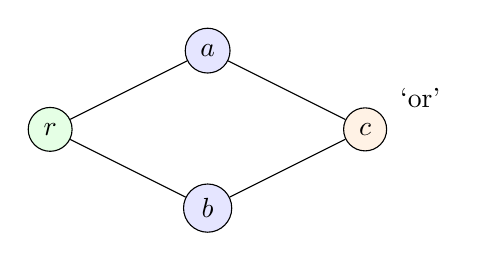
\begin{tikzpicture}
    \node[draw, circle, fill=green!10] (r) at (0, 0) {$r$};

    \node[draw, circle, fill=blue!10] (a) at (2, 1) {$a$};

    \node[draw, circle, fill=blue!10] (b) at (2, -1) {$b$};


    \node[draw, circle, fill=orange!10] (c) at (4, 0) {$c$};

    \node[] (c-or) at (4.7, 0.4) {`or'};

    \draw[-] (r) -- (a);
    \draw[-] (r) -- (b);

    \draw[-] (c) -- (a);
     \draw[-] (c) -- (b);

    
\end{tikzpicture}
        \caption{}\label{subfig:diff-svo}
    \end{subfigure}
    \begin{subfigure}{0.49\linewidth}
      \centering
\begin{tikzpicture}
    % \node[draw, circle, fill=green!10] (r) at (0, 0) {$r$};

    \node[draw, circle, fill=blue!10] (a) at (2, 1) {$a$};

    \node[draw, circle, fill=blue!10] (b) at (2, -1) {$b$};


    \node[draw, circle, fill=orange!10] (c) at (4, 0) {$c$};

    % \draw[-Latex] (r) -- (a);
    % \draw[-Latex] (r) -- (b);

     \node[] (c-or) at (4.7, 0.4) {`and'};

    \draw[-Latex] (a) -- (c);
     \draw[-Latex] (b) -- (c);

    
\end{tikzpicture}
        \caption{}\label{subfig:diff-h2le}
    \end{subfigure}
    \caption{Illustration of the duality between \emph{rooted} $\mathsf{SVO}$ and $\mathsf{LE}$: $(r, a,c,b)$ is a valid SVO, but $(a,c,b)$ is not a valid linear extension.}
    \label{fig:difference}
\end{figure}

Second, we resolve a conjecture of Felsner and Manneville~\cite{FelsnerManneville} by proving $\sharpP$-hardness for counting linear extensions of \defn{N-free} posets of height $3$ (a poset is said to be N-free if its Hasse diagram does not contain the `N' pattern displayed in~\Cref{fig:N-pattern} as an induced subgraph). This conjecture was also recently recorded as open in the survey of Chan and Pak~\cite{LE_survery}. 
\begin{figure}
    \centering
\begin{tikzpicture}
\node[draw, circle, fill=black, inner sep=2pt] (a) at (0,0) {};

\node[draw, circle, fill=black, inner sep=2pt] (b) at (1,0) {};

\node[draw, circle, fill=black, inner sep=2pt] (c) at (0,-1) {};

\node[draw, circle, fill=black, inner sep=2pt] (d) at (1,-1) {};

\draw[-Latex] (d) -- (b);
\draw[-Latex] (d) -- (a);
\draw[-Latex] (c) -- (a);

\end{tikzpicture}
    \caption{The `N' pattern.}
    \label{fig:N-pattern}
\end{figure}

There are several characterizations of N-free posets.
To apply our technique to this problem, we will use the following graph-theoretic formulation. Given a directed acyclic graph $A$, its \defn{edge poset} $P_E(A)$ has one element for each edge of $A$, and for every pair of edges $e_1, e_2$, we set $e_1 \preceq e_2$ whenever $A$ contains a directed path whose first edge is $e_1$ and whose last edge is $e_2$. Thus, a linear extension of $P_E(A)$ is an ordering of the edges of $A$ that is consistent with their precedence along directed paths. In this case, the height of the poset $P_E(A)$ corresponds to the maximum number of edges in a directed path of $A$. A classical characterization states that a poset $P$ is N-free if and only if $P = P_E(A)$ for some directed acyclic graph $A$~\cite{FelsnerManneville}. 



\begin{thm}\label{thm:nfree}
Given an N-free poset of height $3$, it is $\#\mathsf{P}$-complete to count its number of linear extensions.
\end{thm}

There is also a natural duality between shellings of undirected graphs and linear extensions of edge posets, as the former imposes a disjunctive condition over edge orderings, while the latter imposes a conjunctive condition. As we will see, the proofs of \Cref{thm:shellings} and \Cref{thm:nfree} reflect that duality.


\section{Proof Strategy} \label{sec:strategy}

\subsection{Basic Notation}
Given a positive integer $n$, we write $[n]$ to denote the set $\{1, 2, \dots, n\}$. For a finite set $X$, we denote by $X!$ the set of all permutations of $X$. 

\vspace{1em}

To prove our results, we will reduce from the counting version of the exact 3-cover problem ($\mathsf{X3C}$) for which $\mathsf{NP}$-hardness of the decision version is well known. In $\mathsf{X3C}$, we are given a collection of sets $\mathcal{S} := \{S_1, \dots, S_n\}$, each of which consists of $3$ elements from a universe $U := \{u_1, \dots, u_{3h}\}$, and the question is whether we can select exactly $h$ sets from $\mathcal{S}$ such that their union equals $U$. It is well known that $\#\mathsf{X3C}$ is $\#\mathsf{P}$-complete, even under parsimonious reductions \cite{X3C}.
\begin{ex}\label{ex:x3c}For $h=2$, consider a universe $U := \{u_1, \ldots, u_6\}$, and $n=4$ sets
\[
    S_1 = \{u_1, u_2, u_4\}, \; S_2 = \{u_3, u_4, u_6\}, \; S_3 = \{u_1, u_2, u_5\}, \; S_4 = \{u_2, u_5, u_6\}.
\]
Then, $\{S_2, S_3\}$ is a solution, as illustrated in~\Cref{fig:example-a}.
\end{ex}

We will assume that every element $u \in U$ appears in at least one set $S_i$, as otherwise the instances of $\#\mathsf{X3C}$ would be trivial. We can also assume without loss of generality that $h < n$: if $h > n$ then there are no solutions, while if $h = n$, the instance can be solved directly.

The proofs of hardness for $\#\mathsf{SVO}$ and $\#\mathsf{Shellings}$ share the same structure. Starting from an instance $I = (\mathcal{S}, U)$ of $\#\mathsf{X3C}$, we construct a family of graphs $G_{I, q}$, indexed by positive integers $q$. The parameter $q$ controls the number of copies of simple gadgets. For example, in the reduction to $\#\mathsf{SVO}$, each element of $U$ is replaced by $q$ distinct copies that are indistinguishable in terms of adjacencies. Thus, increasing $q$ amplifies the contribution of orderings that make many copied elements available early. We can indeed show that some normalized limit of the number of valid orderings of $G_{I, q}$, as $q \to \infty$, recovers the quantity $\#\mathsf{X3C}(I)$.

Importantly, approximating said limit by direct convergence analysis does not yield a polynomial-time reduction. What we do instead is show that the normalized counting function agrees, for all positive integers $q$, with a rational function in $q$ whose denominator is explicitly known and has polynomial degree. Thus, using an oracle for the target counting problem, we can interpolate the numerator of the rational function exactly by evaluating the normalized count for polynomially many positive integer values of $q$. We then extract the value  $\#\mathsf{X3C}(I)$ by evaluating the limit symbolically.

The proofs of hardness for counting linear extensions follow the same interpolation framework. We again construct a family of posets $P_{I,q}$ indexed by positive integers $q$. 
However, we will see that in these reductions, the orderings that encode exact covers actually have a \emph{smaller} asymptotic contribution. Therefore, the desired quantity cannot be recovered by looking at the leading behavior as $q \to \infty$. The key insight is that the interpolation allows us to recover the entire normalized count as a rational function in $q$. Once this rational function has been reconstructed, we can inspect it symbolically at any value of $q$. In this case, the orderings encoding exact covers are detected by a pole at a suitable negative rational value of $q$. Thus, we can isolate the quantity $\#\mathsf{X3C}(I)$ by multiplying by the corresponding vanishing factor and computing the limit algebraically.

A key tool that we will use throughout the entire paper is the well-known hook-length formula for linear extensions of rooted trees (cf.~\cite[Proposition 1]{gaoCountingShellingsComplete2021}). We include a proof for completeness in~Appendix~\ref{subsec:hook_length}.

\begin{lemma}\label{lemma:tree-le}
    Let $T := (V, \preceq)$ be a poset whose Hasse diagram is a rooted tree. For each element $v \in V$, let $T_v := (\{u \in V \mid v \preceq u\}, \preceq)$ be the poset induced by the subtree rooted at $v$.  Then,
    \[
    \#\mathsf{LE}(T) = \frac{|T|!}{\prod_{v \in V} |T_v|}.
    \]
\end{lemma}

\section{Successive Vertex Orderings}

For simplicity, we will first consider the problem of counting \defn{rooted SVOs}, that is, the number $\#\mathsf{SVO}(G; r)$ of SVOs of a graph $G$ whose first vertex is prescribed to be some $r \in V(G)$. We will thus focus on the following.

\begin{thm}\label{thm:main2}
    Given $G$ and $r$, computing
    $\#\mathsf{SVO}(G; r)$ is $\#\mathsf{P}$-hard, even for bipartite graphs.
\end{thm}

Then we show a simple Turing reduction that allows computing the rooted quantity $\#\mathsf{SVO}(G; r)$ using repeated calls to an oracle for the unrooted variant.

Our reduction for proving~\Cref{thm:main2} will construct the following graphs. Given an instance $I = (\mathcal{S}, U)$ of $\#\mathsf{X3C}$, and a natural number $q \geq 1$ we construct a bipartite graph $G_{I, q}$ as follows:
\begin{enumerate}
    \item Create a vertex $\ns_i$ for each $S_i \in \mathcal{S}$.
    \item Create a root vertex $r$, and connect it to each of the vertices $\ns_1, \dots, \ns_n$.
    \item For each element $u_i \in U$, create $q$ copies $u_i^{(1)}, \dots, u_i^{(q)}$, and connect all copies to every $\ns_j$ such that $u_i \in S_j$.
\end{enumerate} 

An illustration is presented in~\Cref{fig:example-b}. Recall that we are assuming that every element $u \in U$ appears in at least one set $S_i$, and this ensures that our constructed graphs are connected. 

We can already describe how~\Cref{cor:st-numberings} will be obtained from our proof. Let $\widetilde{G}_{I, q}$ be the graph obtained by adding to $G_{I, q}$ an additional vertex $t$ connected to every vertex of $G_{I, q}$. Then, simply note that $\#\mathsf{SVO}(G_{I, q}; r) = \#st\text{-numberings}(\widetilde{G}_{I, q};\, r;\, t)$.

\begin{figure}
    \begin{subfigure}{0.49\linewidth}
         \centering
\begin{tikzpicture}[scale=0.7]
\node[draw, circle, fill=blue!10] (s0) at (2, 7*1.5- 1.5*0) {\small $S_1$};
\node[draw, circle, fill=red!30] (s1) at (2, 7*1.5- 1.5*1) {\small $S_2$};
\node[draw, circle, fill=red!30] (s2) at (2, 7*1.5- 1.5*2) {\small $S_3$};
\node[draw, circle, fill=blue!10] (s3) at (2, 7*1.5- 1.5*3) {\small $S_4$};
\node[draw, circle, fill=orange!10, inner sep=1pt] (e1) at (5, 8*1.5- 1.5*0) {\small $u_1$};
\node[draw, circle, fill=orange!10, inner sep=1pt] (e2) at (5, 8*1.5- 1.5*1) {\small $u_2$};
\node[draw, circle, fill=orange!10, inner sep=1pt] (e3) at (5, 8*1.5- 1.5*2) {\small $u_3$};
\node[draw, circle, fill=orange!10, inner sep=1pt] (e4) at (5, 8*1.5- 1.5*3) {\small $u_4$};
\node[draw, circle, fill=orange!10, inner sep=1pt] (e5) at (5, 8*1.5- 1.5*4) {\small $u_5$};
\node[draw, circle, fill=orange!10, inner sep=1pt] (e6) at (5, 8*1.5- 1.5*5) {\small $u_6$};
\begin{scope}[on background layer]
\draw[] (s0) -- (e1);
\draw[] (s0) -- (e2);
\draw[] (s0) -- (e4);
\draw[very thick, red!50!gray] (s1) -- (e3);
\draw[very thick,red!50!gray] (s1) -- (e4);
\draw[very thick,red!50!gray] (s1) -- (e6);
\draw[very thick, red!50!gray] (s2) -- (e1);
\draw[very thick, red!50!gray] (s2) -- (e2);
\draw[very thick, red!50!gray] (s2) -- (e5);
\draw[] (s3) -- (e2);
\draw[] (s3) -- (e5);
\draw[] (s3) -- (e6);
\end{scope}
\end{tikzpicture}

    \caption{Instance $I$ from~Example~\ref{ex:x3c}, with the solution $\{S_2, S_3\}$ colored.}\label{fig:example-a}
    \end{subfigure}
    \hfill
    \begin{subfigure}{0.49\linewidth}
        \centering
\begin{tikzpicture}[scale=0.7]
\node[draw, circle, fill=green!10] (r) at (0, 10.5 - 1.5*1.5) {$r$};
\node[draw, circle, fill=blue!10] (s0) at (2, 7*1.5- 1.5*0) {\small $\ns_1$};
\node[draw, circle, fill=blue!10] (s1) at (2, 7*1.5- 1.5*1) {\small $\ns_2$};
\node[draw, circle, fill=blue!10] (s2) at (2, 7*1.5- 1.5*2) {\small $\ns_3$};
\node[draw, circle, fill=blue!10] (s3) at (2, 7*1.5- 1.5*3) {\small $\ns_4$};
\node[draw, circle, fill=orange!10, inner sep=0pt] (e1_0) at (5.5, 12.93) {\tiny $u_1^{1}$};
\node[draw, circle, fill=orange!10, inner sep=0pt] (e1_1) at (5.19, 12.379999999999999) {\tiny $u_1^{2}$};
\node[draw, circle, fill=orange!10, inner sep=0pt] (e1_2) at (5.81, 12.379999999999999) {\tiny $u_1^{3}$};
\node[draw, dotted, very thick, circle, fill=yellow!10, opacity=0.4, inner sep=10pt] (1_top) at (5.5, 12.579999999999998) {};
\node[draw, circle, fill=orange!10, inner sep=0pt] (e2_0) at (5.5, 11.18) {\tiny $u_2^{1}$};
\node[draw, circle, fill=orange!10, inner sep=0pt] (e2_1) at (5.19, 10.629999999999999) {\tiny $u_2^{2}$};
\node[draw, circle, fill=orange!10, inner sep=0pt] (e2_2) at (5.81, 10.629999999999999) {\tiny $u_2^{3}$};
\node[draw, dotted, very thick, circle, fill=yellow!10, opacity=0.4, inner sep=10pt] (2_top) at (5.5, 10.829999999999998) {};
\node[draw, circle, fill=orange!10, inner sep=0pt] (e3_0) at (5.5, 9.43) {\tiny $u_3^{1}$};
\node[draw, circle, fill=orange!10, inner sep=0pt] (e3_1) at (5.19, 8.879999999999999) {\tiny $u_3^{2}$};
\node[draw, circle, fill=orange!10, inner sep=0pt] (e3_2) at (5.81, 8.879999999999999) {\tiny $u_3^{3}$};
\node[draw, dotted, very thick, circle, fill=yellow!10, opacity=0.4, inner sep=10pt] (3_top) at (5.5, 9.079999999999998) {};
\node[draw, circle, fill=orange!10, inner sep=0pt] (e4_0) at (5.5, 7.68) {\tiny $u_4^{1}$};
\node[draw, circle, fill=orange!10, inner sep=0pt] (e4_1) at (5.19, 7.13) {\tiny $u_4^{2}$};
\node[draw, circle, fill=orange!10, inner sep=0pt] (e4_2) at (5.81, 7.13) {\tiny $u_4^{3}$};
\node[draw, dotted, very thick, circle, fill=yellow!10, opacity=0.4, inner sep=10pt] (4_top) at (5.5, 7.33) {};
\node[draw, circle, fill=orange!10, inner sep=0pt] (e5_0) at (5.5, 5.93) {\tiny $u_5^{1}$};
\node[draw, circle, fill=orange!10, inner sep=0pt] (e5_1) at (5.19, 5.38) {\tiny $u_5^{2}$};
\node[draw, circle, fill=orange!10, inner sep=0pt] (e5_2) at (5.81, 5.38) {\tiny $u_5^{3}$};
\node[draw, dotted, very thick, circle, fill=yellow!10, opacity=0.4, inner sep=10pt] (5_top) at (5.5, 5.58) {};
\node[draw, circle, fill=orange!10, inner sep=0pt] (e6_0) at (5.5, 4.18) {\tiny $u_6^{1}$};
\node[draw, circle, fill=orange!10, inner sep=0pt] (e6_1) at (5.19, 3.63) {\tiny $u_6^{2}$};
\node[draw, circle, fill=orange!10, inner sep=0pt] (e6_2) at (5.81, 3.63) {\tiny $u_6^{3}$};
\node[draw, dotted, very thick, circle, fill=yellow!10, opacity=0.4, inner sep=10pt] (6_top) at (5.5, 3.83) {};
\begin{scope}[on background layer]
\draw[] (r) -- (s0);
\draw[] (r) -- (s1);
\draw[] (r) -- (s2);
\draw[] (r) -- (s3);
\draw[very thick, gray!70] (s0) -- (1_top);
\draw[very thick, gray!70] (s0) -- (2_top);
\draw[very thick, gray!70] (s0) -- (4_top);
\draw[very thick, gray!70] (s1) -- (3_top);
\draw[very thick, gray!70] (s1) -- (4_top);
\draw[very thick, gray!70] (s1) -- (6_top);
\draw[very thick, gray!70] (s2) -- (1_top);
\draw[very thick, gray!70] (s2) -- (2_top);
\draw[very thick, gray!70] (s2) -- (5_top);
\draw[very thick, gray!70] (s3) -- (2_top);
\draw[very thick, gray!70] (s3) -- (5_top);
\draw[very thick, gray!70] (s3) -- (6_top);
\end{scope}
\end{tikzpicture}

    \caption{$G_{I, 3}$. Thick gray edges between a vertex $S_i$ and a ``group'' $U_j := \{u_j^1, u_j^2, u_j^3\}$ represent all edges $\{S_i, u_j^k\}$ for $k \in \{1,2,3\}$.}\label{fig:example-b}
    \end{subfigure}  
    \caption{Illustrations of an instance of $\mathsf{X3C}$ and one of its corresponding graphs.}\label{fig:example}
\end{figure}

We now explain how to compute $\#\mathsf{X3C}(I)$ in polynomial time using queries to $\#\mathsf{SVO}(G_{I,q}; r)$ for different values of $q$, thereby proving~\Cref{thm:main2}. Recall that $I=(\mathcal{S},U)$ is an instance of $\#\mathsf{X3C}$ of the form described in the previous section. Moreover, we write $U(I)$ for the universe of $I$.

Given a fixed permutation $\sigma \in [n]!$, which induces an ordering $\ns_{\sigma(1)}, \ldots, \ns_{\sigma(n)}$ of the vertices $\ns_1, \dots, \ns_n$, we consider the number $\#\mathsf{SVO}(G_{I, q}; r)_{\sigma}$ of SVOs of $G_{I, q}$ whose first vertex is $r$ and for which the induced order on the vertices $\ns_1, \dots, \ns_n$ corresponds to the one induced by $\sigma$. We will now state a combinatorial lemma regarding those numbers.
 
\begin{lemma}\label{lemma:svo-formula}
Let $\sigma \in [n]!$. For each $j \in [n]$, let $c_j(\sigma)$ be the number of elements of $U(I)$ whose earliest covering set is $S_{\sigma(j)}$, that is, those that are covered by $S_{\sigma(j)}$ but are not covered by $S_{\sigma(i)}$ for any $i<j$. Then 
\[
    \#\mathsf{SVO}(G_{I, q}; r)_{\sigma} =  \frac{(n+3hq)!}{\prod_{i=1}^n\left( i + \sum_{j=1}^{i} q\cdot c_{n-j+1}(\sigma)\right)}.
    \]
\end{lemma}

\begin{proof}
 We define a poset $T_{\sigma} := (V(G_{I, q}) \setminus \{r\}, \preceq)$ whose underlying graph is a rooted tree by the following relationships:
\begin{enumerate}
    \item $s_{\sigma(j)} \preceq s_{\sigma(j+1)}$ for every $1 \leq j < n$.
    \item If $S_{\sigma(j)}$ is the earliest set covering element $u$, then $s_{\sigma(j)} \preceq u^{(i)}$ for every $i \in\{1, \ldots, q\}$.
\end{enumerate}
An illustration continuing~\Cref{ex:x3c} is presented in~\Cref{fig:poset-tree}.
Note that $\ns_{\sigma(1)}$ is the root, and that the linear extensions of this poset are exactly the valid $\mathsf{SVO}$s of $G_{I, q}$ (after $r$) that respect $\sigma$. We have that the subtree rooted at $\ns_{\sigma(j)}$ contains exactly $n-j+1$ vertices of the form $\ns_{\sigma(k)}$ for $k \geq j$, and $\sum_{k=j}^n q \cdot c_{k}(\sigma)$ vertices of the form $u^{(i)}$.
Thus, by~\Cref{lemma:tree-le}, we have that
\begin{align*}
    \#\mathsf{SVO}(G_{I, q}; r)_{\sigma} &= \frac{(n+3hq)!}{\prod_{j=1}^n\left((n-j+1) + \sum_{k=j}^n q \cdot c_{k}(\sigma)\right)}\\
    &=  \frac{(n+3hq)!}{\prod_{i=1}^n \left(i + \sum_{j=1}^{i} q\cdot c_{n-j+1}(\sigma)\right)} \tag{changing variables}.
\end{align*}
\end{proof}

\begin{figure}
    \centering
\begin{tikzpicture}[scale=0.7]
\node[draw, circle, fill=blue!10, ] (S_2) at (0*5.0, -0.0) {$S_2$};
\node[draw, circle, fill=blue!10, ] (S_4) at (1*5.0, -0.0) {$S_4$};
\node[draw, circle, fill=orange!10, inner sep=1pt] (u_3^{1}) at (1*5.0, -1.5) {\tiny $u_3^{1}$};
\node[draw, circle, fill=orange!10, inner sep=1pt] (u_3^{2}) at (1*5.0-0.4, -2.2) {\tiny $u_3^{2}$};
\node[draw, circle, fill=orange!10, inner sep=1pt] (u_3^{3}) at (1*5.0-0.8, -2.9) {\tiny $u_3^{3}$};
\node[draw, circle, fill=orange!10, inner sep=1pt] (u_4^{1}) at (1*5.0-0.6, -4.2) {\tiny $u_4^{1}$};
\node[draw, circle, fill=orange!10, inner sep=1pt] (u_4^{2}) at (1*5.0-1.0, -4.9) {\tiny $u_4^{2}$};
\node[draw, circle, fill=orange!10, inner sep=1pt] (u_4^{3}) at (1*5.0-1.4, -5.6) {\tiny $u_4^{3}$};
\node[draw, circle, fill=orange!10, inner sep=1pt] (u_6^{1}) at (1*5.0-1.7, -6.9) {\tiny $u_6^{1}$};
\node[draw, circle, fill=orange!10, inner sep=1pt] (u_6^{2}) at (1*5.0-2.2, -7.6) {\tiny $u_6^{2}$};
\node[draw, circle, fill=orange!10, inner sep=1pt] (u_6^{3}) at (1*5.0-2.6, -8.3) {\tiny $u_6^{3}$};
\node[draw, circle, fill=blue!10, ] (S_1) at (2*5.0, -0.0) {$S_1$};
\node[draw, circle, fill=orange!10, inner sep=1pt] (u_2^{1}) at (2*5.0, -1.5) {\tiny $u_2^{1}$};
\node[draw, circle, fill=orange!10, inner sep=1pt] (u_2^{2}) at (2*5.0-0.4, -2.2) {\tiny $u_2^{2}$};
\node[draw, circle, fill=orange!10, inner sep=1pt] (u_2^{3}) at (2*5.0-0.8, -2.9) {\tiny $u_2^{3}$};
\node[draw, circle, fill=orange!10, inner sep=1pt] (u_5^{1}) at (2*5.0-0.6, -4.2) {\tiny $u_5^{1}$};
\node[draw, circle, fill=orange!10, inner sep=1pt] (u_5^{2}) at (2*5.0-1.0, -4.9) {\tiny $u_5^{2}$};
\node[draw, circle, fill=orange!10, inner sep=1pt] (u_5^{3}) at (2*5.0-1.4, -5.6) {\tiny $u_5^{3}$};
\node[draw, circle, fill=blue!10, ] (S_3) at (3*5.0, -0.0) {$S_3$};
\node[draw, circle, fill=orange!10, inner sep=1pt] (u_1^{1}) at (3*5.0, -1.5) {\tiny $u_1^{1}$};
\node[draw, circle, fill=orange!10, inner sep=1pt] (u_1^{2}) at (3*5.0-0.4, -2.2) {\tiny $u_1^{2}$};
\node[draw, circle, fill=orange!10, inner sep=1pt] (u_1^{3}) at (3*5.0-0.8, -2.9) {\tiny $u_1^{3}$};
\begin{scope}[on background layer]
\draw[ rounded corners=3pt, thick, orange, fill=yellow!5, opacity=0.4] (5.6, -1.3) -- (4.9, -0.9) -- (3.6, -3.1) -- (4.3, -3.5) -- cycle;
\draw[ rounded corners=3pt, thick, orange, fill=yellow!5, opacity=0.4] (5.0, -4.0) -- (4.3, -3.6) -- (3.0, -5.8) -- (3.7, -6.2) -- cycle;
\draw[ rounded corners=3pt, thick, orange, fill=yellow!5, opacity=0.4] (3.9, -6.7) -- (3.2, -6.3) -- (1.8, -8.5) -- (2.5, -8.9) -- cycle;
\draw[ rounded corners=3pt, thick, orange, fill=yellow!5, opacity=0.4] (10.6, -1.3) -- (9.9, -0.9) -- (8.6, -3.1) -- (9.3, -3.5) -- cycle;
\draw[ rounded corners=3pt, thick, orange, fill=yellow!5, opacity=0.4] (10.0, -4.0) -- (9.3, -3.6) -- (8.0, -5.8) -- (8.7, -6.2) -- cycle;
\draw[ rounded corners=3pt, thick, orange, fill=yellow!5, opacity=0.4] (15.6, -1.3) -- (14.9, -0.9) -- (13.6, -3.1) -- (14.3, -3.5) -- cycle;
\draw[-Latex] (S_1) -- (S_3);
\draw[-Latex] (S_1) -- (u_1^{1});
\draw[-Latex] (S_1) -- (u_1^{2});
\draw[-Latex] (S_1) -- (u_1^{3});
\draw[-Latex] (S_2) -- (S_4);
\draw[-Latex] (S_2) -- (u_3^{1});
\draw[-Latex] (S_2) -- (u_3^{2});
\draw[-Latex] (S_2) -- (u_3^{3});
\draw[-Latex] (S_2) -- (u_4^{1});
\draw[-Latex] (S_2) -- (u_4^{2});
\draw[-Latex] (S_2) -- (u_4^{3});
\draw[-Latex] (S_2) -- (u_6^{1});
\draw[-Latex] (S_2) -- (u_6^{2});
\draw[-Latex] (S_2) -- (u_6^{3});
\draw[-Latex] (S_4) -- (S_1);
\draw[-Latex] (S_4) -- (u_2^{1});
\draw[-Latex] (S_4) -- (u_2^{2});
\draw[-Latex] (S_4) -- (u_2^{3});
\draw[-Latex] (S_4) -- (u_5^{1});
\draw[-Latex] (S_4) -- (u_5^{2});
\draw[-Latex] (S_4) -- (u_5^{3});
\end{scope}
\end{tikzpicture}

    \caption{Poset $T_\sigma$ for $\sigma = (2, 4, 1, 3)$, coming from the instance $I$ of~\Cref{ex:x3c} with $q = 3$.}
    \label{fig:poset-tree}
\end{figure}

\Cref{lemma:svo-formula} gives us a rational function for each fixed $\sigma \in [n]!$. We thus have that 
\[
        \frac{\#\mathsf{SVO}(G_{I, q}; r)}{(n+3hq)!} = \sum_{\sigma \in [n]!} \chi_{\sigma}(q),
\]
where
\[
    \chi_{\sigma}(q) \coloneqq  \frac{1}{\prod_{i=1}^n \left(i + \sum_{j=1}^i q \cdot c_{n-j+1}(\sigma)\right)}.
\]

We now show that this sum can be recovered in polynomial time from oracle evaluations.

\begin{proposition}\label{prop:compute-polynomials}
   Given an instance $I = (\mathcal{S}, U)$ of $\#\mathsf{X3C}$, and an oracle for $\#\mathsf{SVO}(\cdot;\cdot)$, we can compute in polynomial time (in terms of the size of the instance $I$) two polynomials $R$ and $D$ in canonical form such that the following equality between rational functions holds:
   \[ \sum_{\sigma \in [n]!} \chi_{\sigma}(q) = \frac{R(q)}{D(q)}.
    \]
\end{proposition}

\begin{proof}
%     First, to each vertex $v \in V(G_{I, q}) \setminus \{r\}$, we associate uniformly at random a ``time'' $t(v) \in [0, 1]$. 
%     Letting $N := |V(G_{I, q})| - 1$, we will treat $t$ as a random variable in $[0,1]^N$. 
%     Note that $t$ naturally induces an ordering of the vertices after $r$: $\pi_t = (v_1, \dots, v_N)$ such that $t(v_1) < t(v_2) < \dots < t(v_N)$.\footnote{Since ties have probability $0$, we can safely ignore them.} 
%     Because this process is completely symmetric among all vertices, each vertex ordering occurs with probability $(N!)^{-1}$.  

%     Now, for an element $u$ in the universe $U(I)$, let $M_t(u)$ be the random variable corresponding to the smallest $t(v)$ s.t. $\{u,v\}$ is an edge in $G_{I,q}$. Equivalently, since by construction such $v$ must be one of the $S_i$ vertices coming from $\mathcal{S}(I)$, we can think of $M_t(u)$ as the earliest time assigned to a set containing $u$.
%      Then, observe that for an ordering of the vertices to be an SVO, we need that for each element $u \in U(I)$, all its $q$ copies $u_i$ hold $t(u_i) > M_t(u)$. Thus, letting $t(\mathcal{S}) \in [0,1]^{|\mathcal{S}|}$ denoting the random variable corresponding to the times only for the vertices in $\mathcal{S}$ and similarly for $t(U)$, we have 
%      \begin{align*}
%         P_I(q) &= \Pr_{t(U), t(\mathcal{S})}\left[\pi_t \text{ is an SVO} \right] \\ 
%         &= \Pr_{t(U), t(\mathcal{S})}\left[\bigcap_{u \in U(I), i \in [q]} \{t(u_i) > M_t(u)\}\right] \\ &= \mathbb{E}_{t(\mathcal{S})}\left[\Pr_{t(U)}\left[ \bigcap_{u \in U(I), i \in [q]} \{t(u_i) > M_t(u)\} \,\Bigg\vert\, t(\mathcal{S}) \right] \right].
%      \end{align*}
%      Since conditioned on $t(\mathcal{S})$, the value of $M_t(u)$ is fixed for each $u \in U(I)$, we obtain
%      \[
%          P_I(q) =  \int_{[0,1]^{|\mathcal{S}|}} \prod_{u \in U(I)} (1 - M_t(u))^q \; \mathrm{d}t.
%      \]
%      Now, up to a set of measure $0$, we can write $[0,1]^{|\mathcal{S}|} = [0,1]^n$ as the disjoint union of $n!$ simplices of the form \[ \Delta_\sigma := \{ 0 < t(S_{\sigma(1)}) < t(S_{\sigma(2)}) < \dots < t(S_{\sigma(n)}) < 1\},\] one for each permutation $\sigma$ of $[n]$.
%      Under this perspective, for a given permutation $\sigma$ and index $j \in [n]$ let 
%      \[
%         c_j(\sigma) := \left| S_{\sigma(j)} \setminus \bigcup_{i=1}^{j-1} S_{\sigma(i)} \right|. 
%      \]
%      In other words, $c_j(\sigma)$ is the number of elements of $U(I)$ whose earliest covering set is $S_{\sigma(j)}$.
%      Then, note that $0 \leq c_j(\sigma) \leq 3$, and $\sum_{j=1}^n c_j(\sigma) = |U(I)|$.
%      Furthermore, for a given $\sigma$, over the simplex $\Delta_\sigma$ we have 

%      \[
%          \prod_{u \in U(I)} (1 - M_t(u))^q  = \prod_{i=1}^n (1 - t(S_{\sigma(i)}))^{q \cdot c_i(\sigma)}.
%      \]
%      Therefore, we can rewrite $P_I(q)$ as
%      \[
%         P_I(q) = \sum_{\sigma \in [n]!} \int_{\Delta_\sigma} \prod_{i=1}^n (1 - t(S_{\sigma(i)}))^{q \cdot c_i(\sigma)} \; \mathrm{d}t.
%      \]

%      Now, we will need the following fact regarding such simplex integrals. 
%      \begin{lemma}\label{lemma:integrals}
%     Let $n \in \mathbb{N}_{\geq 1}$, and let $\beta_1, \dots, \beta_n$ be arbitrary non-negative reals. Then,
%     \[
%         \int_{0 < y_1 < \dots < y_n < 1} \prod_{i=1}^n y_i^{\beta_i} \mathrm{d}\vec{y} = \prod_{i=1}^n \frac{1}{ i +\sum_{j=1}^i \beta_j}.
%     \]
% \end{lemma}
% \noindent

% By \Cref{lemma:svo-formula} we know that

% \[
%         \frac{\#\mathsf{SVO}(G_{I, q}; r)}{(n+3hq)!} = \sum_{\sigma \in [n]!} \chi_{\sigma}(q),
% \]
% where
% \[
%     \chi_{\sigma}(q) \coloneqq  \frac{1}{\prod_{i=1}^n \left(i + \sum_{j=1}^i q \cdot c_{n-j+1}(\sigma)\right)}.
% \]

Note that all terms $i + \sum_{j=1}^i q \cdot c_{n-j+1}(\sigma)$ in the denominator of $\chi_{\sigma}(q)$ are of the form $Cq + \ell$ for integers $0 \leq C \leq |U|$ and $1 \leq \ell \leq n$. Thus, 
the polynomial 
\[
    D(q) := \prod_{C = 0}^{|U|} \prod_{\ell=1}^{n} (Cq + \ell)^n
\]
is necessarily divisible by the polynomial $\frac{1}{\chi_\sigma(q)}$ for every $\sigma$, making $D(q) \cdot \chi_\sigma(q)$ a polynomial of degree at most $\deg D \leq |U|n^2$. Therefore,
\[
    \sum_{\sigma \in [n]!} D(q)\cdot \chi_\sigma(q) = D(q) \cdot \sum_{\sigma \in [n]!} \chi_\sigma(q)
\] is also a polynomial, $R(q)$, of degree at most $|U| \cdot n^2$.  Thus, we can obtain its coefficients by first evaluating $\frac{\#\mathsf{SVO}(G_{I, q}; r)}{(n+3hq)!}$ at the points $1, 2, \ldots, |U|n^2 + 1$ (via the oracle) and $D$ at the same points (directly, since we know $D$ explicitly), then applying Lagrange interpolation, and finally putting the result into canonical form. Notice that $D$ can also be put into canonical form in polynomial time.
\end{proof}

The next proposition shows how to recover $\#\mathsf{X3C}$ from the rational function.

\begin{proposition}\label{prop:reduction}
    % Let $I = (\mathcal{S}, U)$ be an instance of $\#\mathsf{X3C}$ with $|U| = 3h$, and let $R$ and $D$ be the polynomials given by \Cref{prop:compute-polynomials}. Then,
    For every instance $I = (\mathcal{S}, U)$ of $\#\mathsf{X3C}$ with $|U| = 3h$ it holds that
    \[
        \lim_{q \to \infty} q^h \cdot \sum_{\sigma \in [n]!} \chi_{\sigma}(q) = 3^{-h} \cdot \#\mathsf{X3C}(I).
    \]
\end{proposition}

\begin{proof}
% Again using \Cref{lemma:svo-formula}, we have that 

% \[
%         \frac{R(q)}{D(q)} = \sum_{\sigma \in [n]!} \chi_{\sigma}(q),
% \]
% where
% \[
%     \chi_{\sigma}(q) \coloneqq \prod_{i=1}^n \frac{1}{i + \sum_{j=1}^i q \cdot c_{n-j+1}(\sigma)}.
% \]
Define $C_{i, \sigma} := \sum_{j=1}^i c_{n-j+1}(\sigma)$, which corresponds to the number of elements of $U(I)$ whose earliest covering set appears within the last $i$ sets according to $\sigma$. We thus have that
\[
    \chi_{\sigma}(q) = \prod_{i=1}^n \frac{1}{i + q \cdot C_{i, \sigma}}.
\]

We first consider the case where the first $h$ sets according to $\sigma$ form an exact 3-cover, so that $C_{i, \sigma} = 0$ when $i \leq n-h$, and $C_{i, \sigma} = 3(i+h-n)$ when $n-h < i \leq n$. Now observe that
\begin{align*}
\lim_{q \to \infty} q^h \chi_{\sigma}(q) &= \lim_{q \to \infty} q^h \prod_{i=1}^n \frac{1}{i + q C_{i, \sigma}} \\ &= \frac{1}{(n-h)!} \cdot \prod_{i=n-h+1}^n\lim_{q \to \infty} \frac{q}{i+3q(i+h-n)} \\
&= \frac{1}{(n-h)!} \cdot \prod_{i=n-h+1}^n\frac{1}{3(i+h-n)} \\
&= \frac{3^{-h}}{(n-h)!h!}.
\end{align*}
We now consider the case where the first $h$ sets according to $\sigma$ do not form an exact 3-cover, so that $C_{i, \sigma} > 0$ for all $i \geq n-h$. Then we have that
\begin{align*}
0 \leq \lim_{q \to \infty} q^h \chi_{\sigma}(q) &= \lim_{q \to \infty} q^h \prod_{i=1}^n \frac{1}{i + q C_{i, \sigma}}\\
&=
\lim_{q \to \infty}\left(\prod_{i=1}^{n-h-1} \frac{1}{i+qC_{i, \sigma}}\right) \cdot \frac{1}{n-h + qC_{n-h, \sigma}}\cdot \left(\prod_{i=n-h+1}^n \frac{q}{i + q C_{i, \sigma}}\right)
\\ &\leq \frac{1}{(n-h-1)!} \cdot \left(\lim_{q \to \infty} \frac{1}{n-h+qC_{n-h, \sigma}} \right) \cdot \prod_{i=n-h+1}^n\lim_{q \to \infty} \frac{q}{i+qC_{i, \sigma}} \\
&= \frac{1}{(n-h-1)!} \cdot 0 \cdot \prod_{i=n-h+1}^n\frac{1}{C_{i, \sigma}} \\
&= 0.
\end{align*}
Let $X \subseteq [n]!$ be the set of permutations $\sigma$ such that the sets $S_{\sigma(1)}, \dots, S_{\sigma(h)}$ form an exact cover. Notice that each exact cover corresponds with exactly $(n-h)!h!$ permutations in $X$. Therefore,
\[
\lim_{q \to \infty} q^h \cdot \sum_{\sigma \in [n]!} \chi_{\sigma}(q) = \sum_{\sigma \in [n]!} \lim_{q \to \infty} q^h \chi_{\sigma}(q) = \sum_{\sigma \in X}{\frac{3^{-h}}{(n-h)!h!}} = 3^{-h} \cdot \#\mathsf{X3C}(I).
\]    
\end{proof}

With these ingredients, the proof of~\Cref{thm:main2} is straightforward.
\begin{proof}[Proof of~\Cref{thm:main2}]
    Let $I$ be an arbitrary instance of $\#\mathsf{X3C}$.
    By~\Cref{prop:compute-polynomials} and ~\Cref{prop:reduction}, we can compute in polynomial time polynomials $R$ and $D$ such that
    \[
        \#\mathsf{X3C}(I) = 3^h \cdot \lim_{q \to \infty} \frac{q^h R(q)}{D(q)}.
    \]
    Since $\frac{q^hR(q)}{D(q)}$ is a ratio of polynomials, of size polynomial in the size of $I$, the limit can be computed symbolically in polynomial time, as it corresponds simply to the ratio of the leading coefficients.
\end{proof}

We will now show how to obtain~\Cref{thm:main} from~\Cref{thm:main2}. The result follows directly from the following proposition.

\begin{proposition}\label{prop:unrooting_SVO}
Given a bipartite graph $G = (V, E)$ and a vertex $r \in V$, it is possible to compute $\#\mathsf{SVO}(G; r)$ in polynomial time, given access to an oracle for counting SVOs of bipartite graphs.
\end{proposition}

\begin{proof}[Proof of~\Cref{prop:unrooting_SVO}]
    % Let $(G, r)$ be an instance of $\#\mathsf{SVO}(G; r)$, and let $n = |V(G)|$. Consider the graph $G_{r, m}$ obtained by replacing the vertex $r$ with a clique $\{r_1, \dots, r_m\}$ and replacing any edge $\{u, r\} \in E$ with the edges $\{u, r_1\}, \dots, \{u, r_m\}$. In particular, $G_{r, 1} = G$. For each $1 \leq i \leq n$, let $c_i$ be the number of SVOs of G such that the vertex $r$ is at position $i$. In particular, $c_1 = \#\mathsf{SVO}(G; r)$.
    
    % We claim that the following equality holds:
    % \begin{equation} \label{root_interpolation}
    % \frac{\#\mathsf{SVO}(G_{r, m})}{m!} = \sum_{i = 1}^n\binom{n-i+\ell-1}{\ell-1}c_i.
    % \end{equation}

    Let $(G; r)$ be an instance of $\#\mathsf{SVO}(G; r)$, where $G$ is bipartite, and let $N = |V(G)|$. We construct another bipartite graph $H_\ell$ by adding $\ell$ additional vertices to $G$, all of which are exclusively connected to $r$. We call these vertices the \emph{leaves} of $H_\ell$.
    Now, observe that there are only two kinds of SVOs for $H_\ell$: those that start with a leaf, and those that do not.
    For the first kind, we claim that their number is
    \[
    \ell \cdot \# \mathsf{SVO}(G; r) \cdot \binom{\ell+N-2}{\ell-1} (\ell-1)!.
    \]
    Indeed, there are $\ell$ options for the initial leaf, after which the only possibility is to place $r$. The remaining ordering, when projected down to $V(G)$, must be an SVO of $G$. The $\ell-1$ remaining leaves can be placed in any of the remaining $\ell+N-2$ positions, in any of their $(\ell-1)!$ possible permutations.

    For the second kind, given an SVO $\pi$ of $G$, let $\pi_r$ be the position of $r$ in $\pi$. Then, $\pi$ can be extended to an SVO of $H_\ell$ by adding the $\ell$ leaves in any of the $\ell+N - \pi_r$ positions after $r$, in any of their $\ell!$ permutations. Therefore, the second kind is counted by
    \[
    \sum_{\pi \in \mathsf{SVO}(G)} \binom{\ell+N - \pi_r}{\ell} \cdot \ell!
    \]
    We can separate the case $\pi_r = 1$, and obtain
    \[
    \sum_{\pi \in \mathsf{SVO}(G)} \binom{\ell+N - \pi_r}{\ell} \cdot \ell! = \# \mathsf{SVO}(G; r) \cdot \binom{\ell+N-1}{\ell} \cdot \ell! + \sum_{\substack{\pi \in \mathsf{SVO}(G)\\ \pi_r > 1}} \binom{\ell+N - \pi_r}{\ell} \cdot \ell!
    \]
    Therefore,
    \[
    \frac{\#\mathsf{SVO}(H_\ell)}{\ell!} = \# \mathsf{SVO}(G; r)\left[\binom{\ell+N-2}{\ell-1} +  \binom{\ell+N-1}{\ell} \right] + \sum_{\substack{\pi \in \mathsf{SVO}(G)\\ \pi_r > 1}} \binom{\ell+N - \pi_r}{\ell}.
    \]
    Now, observe that the right side of the previous equation is a polynomial in $\ell$, whose degree is at most $N-1$. Therefore, by evaluating 
    \[
    \frac{\#\mathsf{SVO}(H_1)}{1!}, \frac{\#\mathsf{SVO}(H_2)}{2!}, \dots, \frac{\#\mathsf{SVO}(H_{N})}{N!}
    \]
    via an oracle for $\#\mathsf{SVO}(\cdot)$, and using Lagrange interpolation, we recover the coefficients of the polynomial in canonical form
    \[
    P(\ell) := \# \mathsf{SVO}(G; r)\left[\binom{\ell+N-2}{\ell-1} +  \binom{\ell+N-1}{\ell} \right] + \sum_{\substack{\pi \in \mathsf{SVO}(G)\\ \pi_r > 1}} \binom{\ell+N - \pi_r}{\ell}.
    \]
    But the leading coefficient of this polynomial is precisely $\frac{2}{(N-1)!}\#\mathsf{SVO}(G; r)$. Therefore, we have shown that polynomially many queries to an oracle for $\#\mathsf{SVO}(\cdot)$ allow us to compute $\#\mathsf{SVO}(G; r)$, and thus by~\Cref{thm:main2} we conclude the proof.
\end{proof}

\section{Linear Extensions of Height-2 Posets}

% Let $c_{j}(\sigma)$ be the number of elements of $U(I)$ whose \emph{last} covering set is $S_{\sigma(j)}$. We again have $\sum_{j=1}^n c_j(\sigma) = |U(I)|$, 
% and similarly, 
% \[
%         P_I(q) = \sum_{\sigma \in [n]!} \int_{\Delta_\sigma} \prod_{i=1}^n (1 - t(S_{\sigma(i)}))^{q \cdot c_i(\sigma)} \; \mathrm{d}t.
%      \]
% By the same~\Cref{lemma:integrals}, we get that the integral over the simplex induced by $\sigma$ evaluates to
% \[
%     \chi_{\sigma}(q) := \prod_{i=1}^n \frac{1}{i + \sum_{j=1}^i q \cdot c_{n-j+1}(\sigma)}.
% \]

We again reduce from $\#\mathsf{X3C}$. The gadgets are essentially the same as the ones we used for proving hardness of $\#\mathsf{SVO}$. Given an instance $I = (\mathcal{S}, U)$ of $\#\mathsf{X3C}$, and a natural number $q \geq 1$ we construct a poset $P_{I, q}$ of height $2$ as follows:
\begin{enumerate}
    \item Create an element $\ns_i$ of the first layer for each $S_i \in \mathcal{S}$.
    \item For each element $u_i \in U$, create $q$ copies $u_i^{(1)}, \dots, u_i^{(q)}$ and add all the relations $\ns_j < u_i^{(k)}$ such that $u_i \in S_j$.
\end{enumerate} 

Given a fixed permutation $\sigma \in [n]!$, which induces an ordering $\ns_{\sigma(1)}, \ldots, \ns_{\sigma(n)}$ of the elements of the first layer, we consider the number $\#\mathsf{LE}(P_{I, q})_{\sigma}$ of linear extensions of $P_{I, q}$ for which the induced order on the elements $\ns_1, \dots, \ns_n$ corresponds to the one induced by $\sigma$.

\begin{lemma}\label{lemma:le-formula}
Let $\sigma \in [n]!$. For each $j \in [n]$, let $c_j(\sigma)$ be the number of elements of $U(I)$ whose last covering set is $S_{\sigma(j)}$, that is, those that are covered by $S_{\sigma(j)}$ but are not covered by $S_{\sigma(i)}$ for any $i>j$. Then 
\[
    \#\mathsf{LE}(P_{I, q})_{\sigma} =  \frac{(n+3hq)!}{\prod_{i=1}^n \left(i + \sum_{j=1}^{i} q\cdot c_{n-j+1}(\sigma)\right)}.
    \]
\end{lemma}

\begin{proof}
 We define a new poset $T_{\sigma}$ over the same elements but a new relation $\preceq$ given by the following conditions:
\begin{enumerate}
    \item $\ns_{\sigma(j)} \preceq \ns_{\sigma(j+1)}$ for every $1 \leq j < n$.
    \item If $S_{\sigma(j)}$ is the last set covering element $u$, then $\ns_{\sigma(j)} \preceq u^{(i)}$ for every $i \in \{1, \ldots, q\}$.
\end{enumerate}
Note that $T_{\sigma}$ is a tree poset, and its linear extensions are exactly the valid linear extensions of $P_{I, q}$ that respect $\sigma$. We have that the subtree rooted at $\ns_{\sigma(j)}$ contains exactly $n-j+1$ elements of the form $\ns_{\sigma(k)}$ for $k \geq j$, and $\sum_{k=j}^n q \cdot c_{k}(\sigma)$ elements of the form $u^{(i)}$.
Thus, by~\Cref{lemma:tree-le}, we have that
\begin{align*}
    \#\mathsf{LE}(P_{I, q})_{\sigma} &= \frac{(n+3hq)!}{\prod_{j=1}^n \left((n-j+1) + \sum_{k=j}^n q \cdot c_{k}(\sigma)\right)}\\
    &=  \frac{(n+3hq)!}{\prod_{i=1}^n \left(i + \sum_{j=1}^{i} q\cdot c_{n-j+1}(\sigma)\right)} \tag{change variables}.
\end{align*}
\end{proof}

From \Cref{lemma:le-formula} it follows that

\[
        \frac{\#\mathsf{LE}(P_{I, q})}{(n+3hq)!} = \sum_{\sigma \in [n]!} \chi_{\sigma}(q),
\]
where
\[
    \chi_{\sigma}(q) \coloneqq \frac{1}{\prod_{i=1}^n  \left(i + \sum_{j=1}^i q \cdot c_{n-j+1}(\sigma)\right)}.
\]


As before, we now show how to recover that sum in polynomial time from oracle evaluations.

\begin{proposition}\label{prop:le_compute-polynomials}
   Given an instance $I$ of $\#\mathsf{X3C}$, and an oracle for $\#\mathsf{LE}(\cdot)$, we can compute in polynomial time (in terms of the size of the instance $I$) two polynomials $R$ and $D$ in canonical form such that the following equality between rational functions holds:
   \[ \sum_{\sigma \in [n]!} \chi_{\sigma}(q) = \frac{R(q)}{D(q)}.
    \]
\end{proposition}

\begin{proof}
The argument will be completely analogous to the proof of \Cref{prop:compute-polynomials}.
% By \Cref{lemma:le-formula} we know that

% \[
%         \frac{\#\mathsf{LE}(P_{I, q})}{(n+3hq)!} = \sum_{\sigma \in [n]!} \chi_{\sigma}(q),
% \]
% where
% \[
%     \chi_{\sigma}(q) \coloneqq \frac{1}{\prod_{i=1}^n  \left(i + \sum_{j=1}^i q \cdot c_{n-j+1}(\sigma)\right)}.
% \]
Note that all terms $i + \sum_{j=1}^i q \cdot c_{n-j+1}(\sigma)$ are of the form $Cq + \ell$ for integers $0 \leq C \leq |U|$ and $1 \leq \ell \leq n$. Thus, 
the polynomial 
\[
    D(q) := \prod_{C = 0}^{|U|} \prod_{\ell=1}^{n} (Cq + \ell)^n
\]
is divisible by the polynomial $\frac{1}{\chi_\sigma(q)}$ for every $\sigma$, making $D(q) \cdot \chi_\sigma(q)$ a polynomial of degree at most $\deg D \leq |U|n^2$. Therefore,
\[
    \sum_{\sigma \in [n]!} D(q)\cdot \chi_\sigma(q) = D(q) \cdot \sum_{\sigma \in [n]!} \chi_\sigma(q)
\] is also a polynomial, $R(q)$, of degree at most $|U| \cdot n^2$.  We can obtain its coefficients by evaluating $\frac{\#\mathsf{LE}(P_{I, q})}{(n+3hq)!}$ at the points $1, 2, \ldots, |U|n^2 + 1$ (via the oracle) and $D$ at the same points (directly), then applying Lagrange interpolation, and finally putting the result into canonical form.
\end{proof}

It remains to show how to recover $\#\mathsf{X3C}$ from the rational function.

\begin{proposition}\label{prop:le_limit}
    For every instance $I = (\mathcal{S}, U)$ of $\#\mathsf{X3C}$ with $|U| = 3h$ it holds that
    \[
        \lim_{q \to -\frac{1}{3}} (3q+1)^h  \cdot \sum_{\sigma \in [n]!} \chi_{\sigma}(q) = \#\mathsf{X3C}(I).
    \]
\end{proposition}

\begin{proof}
% Again using \Cref{lemma:le-formula}, we have that 
% \(
%         \frac{R(q)}{D(q)} = \sum_{\sigma \in [n]!} \chi_{\sigma}(q),
% \)
% where
% \[
%     \chi_{\sigma}(q) \coloneqq \prod_{i=1}^n \frac{1}{i + \sum_{j=1}^i q \cdot c_{n-j+1}(\sigma)}.
% \]
Let $C_{i, \sigma} := \sum_{j=1}^i c_{n-j+1}(\sigma)$ be the number of elements whose last covering set appears within the last $i$ sets according to $\sigma$. We thus have
\[
    \chi_{\sigma}(q) =  \prod_{i=1}^n \frac{1}{i + q C_{i, \sigma} }.
\]
% Now, think of permutations $\sigma$ that finish on an exact cover; 
% Thus, for $q \to \frac{-1}{3}$, we have that 
% $i + q C_{i, \sigma} \to 0$ over the last $h$ terms, so it seems that 
% \[
%     \lim_{q \to -\frac{1}{3}} P_I(q)
% \]
% can be somehow expressed in terms of $\#\mathsf{X3C}(I)$.
Let $\sigma$ be a permutation such that its last $h$ sets are an exact cover. Then, the last $h$ sets are all pairwise disjoint, and thus $C_{i, \sigma} = 3i$ for $1 \leq i \leq h$, and for $i > h$ we simply have $C_{i, \sigma} = 3h$.
Then,
 \begin{align*}
     \lim_{q \to -\frac{1}{3}} (3q+1)^h\chi_{\sigma}(q) &= \lim_{q \to -\frac{1}{3}}  (3q+1)^h \prod_{i=1}^{h} \frac{1}{i + q\cdot 3i }  \cdot \prod_{i=h+1}^{n} \frac{1}{i + q\cdot 3h }\\
     &= \lim_{q \to -\frac{1}{3}}   \prod_{i=1}^{h} \frac{(3q+1)}{i(3q+1)}  \cdot \prod_{i=h+1}^{n} \frac{1}{i + q\cdot 3h }\\
     &= \frac{1}{h!} \lim_{q \to -\frac{1}{3}}  \prod_{i=h+1}^{n} \frac{1}{i + q\cdot 3h }\\
     &= \frac{1}{h!} \prod_{i=h+1}^{n} \lim_{q \to -\frac{1}{3}} \frac{1}{i + q\cdot 3h }\\
     &= \frac{1}{h!} \cdot \prod_{i=h+1}^{n} \frac{1}{i - h } \\
     &= \frac{1}{h! (n-h)!}.
 \end{align*}
 Now let $\sigma$ be a permutation such that its last $h$ sets are \emph{not} an exact cover. Then, define \[B_\sigma := \{ i \in [h] \mid C_{i, \sigma} < 3i \}.\] The fact that the last $h$ sets of $\sigma$ are not an exact cover implies that $|B_\sigma| > 0$.
 We thus have
\begin{align*}
      \lim_{q \to -\frac{1}{3}} (3q+1)^h\chi_{\sigma}(q) &= \lim_{q \to -\frac{1}{3}}  (3q+1)^h \prod_{i \in B_\sigma} \frac{1}{i + q \cdot C_{i, \sigma}}  \cdot \prod_{i \in [h] \setminus B_\sigma} \frac{1}{i + q \cdot 3i}  \cdot \prod_{i=h+1}^{n} \frac{1}{i + q\cdot C_{i, \sigma} }\\
      &= \lim_{q \to -\frac{1}{3}}  (3q+1)^{|B_\sigma|} \prod_{i \in B_\sigma} \frac{1}{i + q \cdot C_{i, \sigma}}  \cdot \prod_{i \in [h] \setminus B_\sigma} \frac{(3q+1)}{i(3q+1)}  \cdot \prod_{i=h+1}^{n} \frac{1}{i + q\cdot C_{i, \sigma} }\\
        &= \left(\prod_{i \in [h] \setminus B_\sigma} \frac{1}{i}\right) \cdot \lim_{q \to -\frac{1}{3}} (3q+1)^{|B_\sigma|} \prod_{i \in B_\sigma} \frac{1}{i + q \cdot C_{i, \sigma}}  \cdot \prod_{i=h+1}^{n} \frac{1}{i + q\cdot C_{i, \sigma} } \\
      &= \left(\prod_{i \in [h] \setminus B_\sigma} \frac{1}{i}\right) \cdot \lim_{q \to -\frac{1}{3}}  (3q+1)^{|B_\sigma|} \cdot \left(\prod_{i \in B_\sigma \cup \{h+1, \dots, n\}} \frac{3}{3i - C_{i, \sigma}}\right)\\
      &= \left(\prod_{i \in [h] \setminus B_\sigma} \frac{1}{i}\right) \cdot 0 \cdot \left(\prod_{i \in B_\sigma \cup \{h+1, \dots, n\}} \frac{3}{3i - C_{i, \sigma}}\right)\\
      &= 0.
\end{align*}
Let $X \subseteq [n]!$ be the set of permutations $\sigma$ whose last $h$ sets form an exact cover. Notice that each exact cover corresponds with exactly $(n-h)!h!$ permutations in $X$. Therefore,
\[
\lim_{q \to -\frac{1}{3}} (3q+1)^h  \cdot \sum_{\sigma \in [n]!} \chi_{\sigma}(q) = \sum_{\sigma \in [n]!} \lim_{q \to -\frac{1}{3}} (3q+1)^h \chi_{\sigma}(q) = \sum_{\sigma \in X}{\frac{1}{(n-h)!h!}} = \#\mathsf{X3C}(I).
\]    
\end{proof}

With these ingredients, we can now give an alternative proof of the following result.

\begin{thm}\label{thm:h2le}
$\#\mathsf{LE}$ is $\#\mathsf{P}$-hard, even for height $2$ posets.
\end{thm}

\begin{proof}[Proof of~\Cref{thm:h2le}]
    Let $I$ be an arbitrary instance of $\#\mathsf{X3C}$.
    By~\Cref{prop:le_compute-polynomials} and ~\Cref{prop:le_limit}, we can compute in polynomial time polynomials $R$ and $D$ such that
    \[
        \#\mathsf{X3C}(I) = \lim_{q \to -\frac{1}{3}} \frac{(3q+1)^h R(q)}{D(q)}.
    \]
    Since
$\frac{(3q+1)^h R(q)}{D(q)}$
is a ratio of polynomials whose size is polynomial in the size of $I$, the limit
$\lim_{q \to -\frac{1}{3}} \frac{(3q+1)^h R(q)}{D(q)}$
can be computed by simply evaluating the numerator and denominator at $q=-\frac{1}{3}$, except when this evaluation yields the indeterminate form $\frac{0}{0}$. In that case, we repeatedly apply L'Hôpital's rule until the resulting limit is no longer of the form $\frac{0}{0}$, after which it can be computed by evaluating the resulting polynomials at $q=-\frac{1}{3}$.
\end{proof}

\section{Shellings}

In this section we prove~\Cref{thm:shellings}. For simplicity, we will first prove a \emph{rooted} version, and then show how to get rid of this assumption. More precisely, we will first consider the function $\#\mathsf{Shellings}(G; r)$ that counts the number of shellings of $G$ whose first edge is incident to the vertex $r$. Thus, we aim to prove the following result.
\begin{thm}\label{thm:shellings2}
Given a bipartite graph $G = (V, E)$ and a vertex $r \in V$, 
computing $\#\mathsf{Shellings}(G; r)$ is $\sharpP$-hard.
\end{thm}

\begin{proof}
    
We reduce again from $\#\mathsf{X3C}$, and let $I = (\mathcal{S}, U)$ be an input instance, with $|\mathcal{S}| = n$ and $|U| = 3h$.
We construct a graph $H_{I, q}$ defined as follows:
\begin{enumerate}
    \item Create a vertex $\ns_i$ for each $S_i \in \mathcal{S}$, and a vertex $\nou_j$ for each $u_j \in U$.
    \item Create an edge $\{\ns_i, \nou_j\}$ whenever $u_j \in S_i$.
    \item Create a vertex $r$ connected to every $\ns_i$.
    \item For each $u_j \in U$, create $q$ additional copies $u_j^{(k)}$ ($1 \leq k \leq q$), and connect them all to $\nou_j$.
\end{enumerate}
An illustration is presented in~\Cref{fig:shellings}. Note that $H_{I, q}$ is always bipartite.
Let $E_q := E(H_{I, q})$,
and let $E' \subsetneq E_q$ be the subset of edges introduced in steps (2) and (3). Note that $|E'| = 4|\mathcal{S}| = 4n$.
Also, for each permutation $\sigma$ of $E'$, we consider the number $\#\mathsf{Shellings}(H_{I, q}; r)_{\sigma}$ of shellings of $H_{I, q}$ whose first edge is incident to $r$ and whose projection down to $E'$ coincides with $\sigma$. We will write $\omsh$ to denote the subset of permutations $\sigma$ of $E'$ for which $\#\mathsf{Shellings}(H_{I, q}; r)_{\sigma} > 0$.

\begin{figure}
    \centering
\begin{tikzpicture}[scale=0.7]
\node[draw, circle, fill=green!10] (r) at (0, 10.5 - 1.5*1.5) {$r$};
\node[draw, circle, fill=blue!10] (s0) at (2, 7*1.5- 1.5*0) {\small $s_1$};
\node[draw, circle, fill=blue!10] (s1) at (2, 7*1.5- 1.5*1) {\small $s_2$};
\node[draw, circle, fill=blue!10] (s2) at (2, 7*1.5- 1.5*2) {\small $s_3$};
\node[draw, circle, fill=blue!10] (s3) at (2, 7*1.5- 1.5*3) {\small $s_4$};
\node[draw, circle, fill=orange!10, inner sep=0pt] (e1_0) at (7.5, 12.93) {\tiny $u_1^{1}$};
\node[draw, circle, fill=orange!10, inner sep=0pt] (e1_1) at (7.19, 12.379999999999999) {\tiny $u_1^{2}$};
\node[draw, circle, fill=orange!10, inner sep=0pt] (e1_2) at (7.81, 12.379999999999999) {\tiny $u_1^{3}$};
\node[draw, circle, fill=orange!30, opacity=0.7, inner sep=2pt] (1_main) at (5.0, 12.579999999999998) {$\nou_1$};
\node[draw, dotted, very thick, circle, fill=yellow!10, opacity=0.4, inner sep=10pt] (1_top) at (7.5, 12.579999999999998) {};
\node[draw, circle, fill=orange!10, inner sep=0pt] (e2_0) at (7.5, 11.18) {\tiny $u_2^{1}$};
\node[draw, circle, fill=orange!10, inner sep=0pt] (e2_1) at (7.19, 10.629999999999999) {\tiny $u_2^{2}$};
\node[draw, circle, fill=orange!10, inner sep=0pt] (e2_2) at (7.81, 10.629999999999999) {\tiny $u_2^{3}$};
\node[draw, circle, fill=orange!30, opacity=0.7, inner sep=2pt] (2_main) at (5.0, 10.829999999999998) {$\nou_2$};
\node[draw, dotted, very thick, circle, fill=yellow!10, opacity=0.4, inner sep=10pt] (2_top) at (7.5, 10.829999999999998) {};
\node[draw, circle, fill=orange!10, inner sep=0pt] (e3_0) at (7.5, 9.43) {\tiny $u_3^{1}$};
\node[draw, circle, fill=orange!10, inner sep=0pt] (e3_1) at (7.19, 8.879999999999999) {\tiny $u_3^{2}$};
\node[draw, circle, fill=orange!10, inner sep=0pt] (e3_2) at (7.81, 8.879999999999999) {\tiny $u_3^{3}$};
\node[draw, circle, fill=orange!30, opacity=0.7, inner sep=2pt] (3_main) at (5.0, 9.079999999999998) {$\nou_3$};
\node[draw, dotted, very thick, circle, fill=yellow!10, opacity=0.4, inner sep=10pt] (3_top) at (7.5, 9.079999999999998) {};
\node[draw, circle, fill=orange!10, inner sep=0pt] (e4_0) at (7.5, 7.68) {\tiny $u_4^{1}$};
\node[draw, circle, fill=orange!10, inner sep=0pt] (e4_1) at (7.19, 7.13) {\tiny $u_4^{2}$};
\node[draw, circle, fill=orange!10, inner sep=0pt] (e4_2) at (7.81, 7.13) {\tiny $u_4^{3}$};
\node[draw, circle, fill=orange!30, opacity=0.7, inner sep=2pt] (4_main) at (5.0, 7.33) {$\nou_4$};
\node[draw, dotted, very thick, circle, fill=yellow!10, opacity=0.4, inner sep=10pt] (4_top) at (7.5, 7.33) {};
\node[draw, circle, fill=orange!10, inner sep=0pt] (e5_0) at (7.5, 5.93) {\tiny $u_5^{1}$};
\node[draw, circle, fill=orange!10, inner sep=0pt] (e5_1) at (7.19, 5.38) {\tiny $u_5^{2}$};
\node[draw, circle, fill=orange!10, inner sep=0pt] (e5_2) at (7.81, 5.38) {\tiny $u_5^{3}$};
\node[draw, circle, fill=orange!30, opacity=0.7, inner sep=2pt] (5_main) at (5.0, 5.58) {$\nou_5$};
\node[draw, dotted, very thick, circle, fill=yellow!10, opacity=0.4, inner sep=10pt] (5_top) at (7.5, 5.58) {};
\node[draw, circle, fill=orange!10, inner sep=0pt] (e6_0) at (7.5, 4.18) {\tiny $u_6^{1}$};
\node[draw, circle, fill=orange!10, inner sep=0pt] (e6_1) at (7.19, 3.63) {\tiny $u_6^{2}$};
\node[draw, circle, fill=orange!10, inner sep=0pt] (e6_2) at (7.81, 3.63) {\tiny $u_6^{3}$};
\node[draw, circle, fill=orange!30, opacity=0.7, inner sep=2pt] (6_main) at (5.0, 3.83) {$\nou_6$};
\node[draw, dotted, very thick, circle, fill=yellow!10, opacity=0.4, inner sep=10pt] (6_top) at (7.5, 3.83) {};
\begin{scope}[on background layer]
\draw[] (r) -- (s0);
\draw[] (r) -- (s1);
\draw[] (r) -- (s2);
\draw[] (r) -- (s3);
\draw[] (s0) -- (1_main);
\draw[very thick, gray!70] (1_main) -- (1_top);
\draw[] (s0) -- (2_main);
\draw[very thick, gray!70] (2_main) -- (2_top);
\draw[] (s0) -- (4_main);
\draw[very thick, gray!70] (4_main) -- (4_top);
\draw[] (s1) -- (3_main);
\draw[very thick, gray!70] (3_main) -- (3_top);
\draw[] (s1) -- (4_main);
\draw[very thick, gray!70] (4_main) -- (4_top);
\draw[] (s1) -- (6_main);
\draw[very thick, gray!70] (6_main) -- (6_top);
\draw[] (s2) -- (1_main);
\draw[very thick, gray!70] (1_main) -- (1_top);
\draw[] (s2) -- (2_main);
\draw[very thick, gray!70] (2_main) -- (2_top);
\draw[] (s2) -- (5_main);
\draw[very thick, gray!70] (5_main) -- (5_top);
\draw[] (s3) -- (2_main);
\draw[very thick, gray!70] (2_main) -- (2_top);
\draw[] (s3) -- (5_main);
\draw[very thick, gray!70] (5_main) -- (5_top);
\draw[] (s3) -- (6_main);
\draw[very thick, gray!70] (6_main) -- (6_top);
\end{scope}
\end{tikzpicture}

    \caption{Illustration of $H_{I, q}$ for $q = 3$.}
    \label{fig:shellings}
\end{figure}

We now define a poset $T_{\sigma} := (E_q, \preceq)$ for each fixed $\sigma \in \omsh$. For ease of notation, let us write $e_1^\sigma, \dots, e_{4n}^\sigma$ for the edges in $E'$ ordered according to $\sigma$. Also, for an element $u_j \in U$, let \[
\rho_{\sigma}(u_j) := \min \{ i \mid e_{i}^\sigma = \{\ns_\ell, \nou_j\} \text{ for some } \ell \}.
\]Intuitively, $\rho_{\sigma}(u_j)$  is the earliest moment in which $\nou_j$ becomes connected to the shelling.
With this notation, the order $\preceq$ is defined by:
\begin{enumerate}
    \item $e_1^\sigma \preceq e_2^\sigma \preceq \dots  \preceq e_{4n-1}^\sigma \preceq e_{4n}^\sigma$.
    \item For each edge $e := \{\nou_j, u_j^{(k)}\} \in E_q \setminus E'$, we have $e_{\rho_\sigma(u_j)}^\sigma \preceq e$.
\end{enumerate}
Because $\sigma \in \omsh$, observe that the linear extensions of $T_\sigma$ are exactly the shellings of $H_{I, q}$ whose first edge is incident to $r$ and whose projection down to $E'$ coincides with $\sigma$. Thus, by~\Cref{lemma:tree-le}, we have
\[
\#\mathsf{Shellings}(H_{I, q}; r)_{\sigma} = (4n+3hq)! \prod_{i=1}^{4n}\frac{1}{i + q \cdot C_{i, \sigma}},
\]
where 
\[ 
C_{i, \sigma} := |\{ u_j \in U \mid   \rho_{\sigma}(u_j) \geq 4n + 1 -i \}|.
\]
Notice that $C_{i, \sigma} \leq C_{j, \sigma}$ whenever $i < j$. 

We now have that
\[
\frac{\#\mathsf{Shellings}(H_{I, q}; r)}{(4n+3hq)!} = \sum_{\sigma \in \omsh} \chi_{\sigma}(q),
\]
where
\[
\chi_{\sigma}(q) \coloneqq \prod_{i=1}^{4n}\frac{1}{i + q \cdot C_{i, \sigma}}.
\]
Now, let us say that a permutation $\sigma \in \omsh$ \emph{induces} an exact cover $X \subseteq \mathcal{S}$ if the first $4h$ edges according to $\sigma$ correspond in some ordering to:
all edges $\{r, \ns_i\}$ for $S_i \in X$, and all edges $\{\ns_i, \nou_j\}$ for $S_i \in X$, $u_j \in S_i$. Let $\omxc \subseteq \omsh$ be the subset of permutations that induce an exact cover. We will need the following claim regarding such permutations.

\begin{claim}\label{claim:cover_characterization}
Given any $\sigma \in \omsh$, the following statements hold:
\begin{enumerate}
\item If $\sigma \in \omxc$, then $C_{4n-4h, \sigma} = 0$ and $C_{4n-4h+1, \sigma} > 0$.
\item If $\sigma \notin \omxc$, then $C_{4n-4h, \sigma} > 0$.
\end{enumerate}
\end{claim}
\begin{proof}[Proof of~\Cref{claim:cover_characterization}]
Let $e_1, \ldots, e_{4n}$ be the edges of $E'$ ordered according to $\sigma$. 

First, suppose that $\sigma$ induces an exact cover $X \subseteq \mathcal{S}$. Then, by definition, the subgraph of $H_{I, q}$ induced by the first $4h$ edges of $\sigma$ already contains all vertices $\nou_j$, and therefore $C_{4n-4h, \sigma} = 0$.
%Note that, since $\sigma$ is a shelling, we have that $|\bigcup_{i=1}^k e_{i}| \leq k+1$ for each $k \in \{1, \ldots, 4n\}$.
Since $X$ is an exact cover, the subgraph of $H_{I, q}$ induced by the vertices
    \(
    \{ r \} \cup \{ \ns_i\ \mid S_i \in X\} \cup \{\nou_j \mid u_j \in U \}
    \)
is a tree. Therefore, since $\sigma$ is a shelling, the edge $e_{4h}$ must be incident to a leaf of that tree. Since $e_1$ is incident to the root $r$, we necessarily have that $e_{4h}$ is of the form $\{\ns_i, \nou_j\}$ for $S_i \in X$ and $u_j \in S_i$. This shows that $C_{4n-4h+1, \sigma} > 0$.

For the second part, we prove the contrapositive. Suppose that $\sigma \in \omsh$ is such that $C_{4n-4h, \sigma} = 0$. Then, the subgraph $H_{\sigma}$ of $H_{I, q}$ induced by the edges $e_1, \dots e_{4h}$ must contain all vertices $\nou_j$ for $u_j \in U$. Now let $Y$ be the set of vertices of the form $\ns_i$ belonging to $H_\sigma$. Because $H_\sigma$ is bipartite and $Y$ is one of the parts, we have that
\begin{equation}\label{eq:degrees}
      4h = \sum_{v \in Y}{\deg_{H_{\sigma}}(v)} \leq \sum_{v \in Y}{\deg_{H_{I, q}}(v)} = \sum_{v \in Y}{4} = 4|Y|,
      \end{equation}
and hence $|Y| \geq h$. On the other hand, since $\sigma$ is a shelling, we have that $H_\sigma$ is connected, and therefore $1+|Y|+3h$, its number of vertices, must be at most $4h+1$, which implies that $|Y| = h$. From equation~\eqref{eq:degrees} it follows that $\deg_{H_{I, q}}(v) = 4$ for every $v \in Y$, which shows that indeed $Y$ corresponds to an exact cover.
\end{proof} 

Now, the first part of \Cref{claim:cover_characterization} implies that, for any $\sigma \in \omxc $, we have $C_{i, \sigma} = 0$ if and only if $i \leq 4n - 4h$. Therefore, for any $\sigma \in \omxc$, we have
\begin{align*}
\lim_{q \to \infty} q^{4h} \chi_{\sigma}(q) &= \lim_{q \to \infty} q^{4h} \prod_{i=1}^{4n} \frac{1}{i + q C_{i, \sigma}} \\ &= \frac{1}{(4n-4h)!} \cdot \prod_{i=4n-4h+1}^{4n}\lim_{q \to \infty} \frac{q}{i+qC_{i, \sigma}}\\
&= \frac{1}{(4n-4h)!} \cdot \prod_{i=4n-4h+1}^{4n}\frac{1}{C_{i,\sigma}}.
\end{align*}

On the other hand, by the second part of \Cref{claim:cover_characterization}, for any $\sigma \in \omsh \setminus \omxc$, we have
\begin{align*}
    0 \leq \lim_{q \to \infty} q^{4h} \chi_{\sigma}(q) &= \lim_{q \to \infty} q^{4h} \left(\prod_{i = 1}^{4n-4h-1} \frac{1}{i + q C_{i, \sigma}}\right) \cdot \left(\prod_{i = 4n-4h}^{4n} \frac{1}{i + q C_{i, \sigma}}\right)\\
    &\leq \lim_{q \to \infty} q^{4h} \left(\prod_{i = 1}^{4n-4h-1} \frac{1}{i}\right) \cdot \left(\prod_{i = 4n-4h}^{4n} \frac{1}{i + q C_{i, \sigma}}\right) \\
    &= \frac{1}{(4n-4h-1)!} \lim_{q \to \infty} q^{-1}  \left(\prod_{i = 4n-4h}^{4n} \frac{q}{i + q C_{i, \sigma}}\right) \\
    &= \frac{1}{(4n-4h-1)!} \cdot \left(\prod_{i = 4n-4h}^{4n} \frac{1}{C_{i, \sigma}}\right) \cdot \lim_{q \to \infty} q^{-1} \\
    &= 0.
\end{align*}

To finish the proof we will rely on the following claim, whose proof uses a probabilistic argument and is deferred to~Appendix~\ref{subsec:claim_shellings}.
\begin{claim}\label{claim:omega-xc}
Fix an exact cover $X \subseteq \mathcal{S}$, and let $\omxc(X) \subseteq \omxc$ be the set of permutations that induce the exact cover $X$. Then,
    \[
\sum_{\sigma \in\omxc(X)} \prod_{t=1}^{4h} \frac{1}{C_{4n-4h+t, \sigma}} = (4n-4h)! \cdot 3^{-h}.
\]
\end{claim}
%
% On the other hand, we will need the following simpler claim regarding permutations that do \emph{not} induce exact covers.
%
% \begin{claim}\label{claim:non-cover}
% Let $\sigma \in \omsh \setminus \omxc$ be a permutation that does not induce an exact cover, and let $A_{\sigma} := \{ i \in [4n] \mid C_{i, \sigma} > 0\}$. Then, $|A_\sigma| \geq 4h+1$.
% \end{claim}
% \begin{proof}[Proof of~\Cref{claim:non-cover}]
%     Let us assume $|A_\sigma| \leq 4h$, and then show that $\sigma$ must induce an exact cover. Let $E_{\sigma}$ be the set containing the first $4h$ edges according to $\sigma$. Then, since $|A_{\sigma}| \leq 4h$, the subgraph $H_{\sigma}$ of $H_{I, q}$ induced by the edges $E_{\sigma}$ must contain all vertices $u \in U$. 
%     Moreover, note that $V(H_\sigma) \cap U \subseteq N(V(H_\sigma) \cap \mathcal{S})$. Since each vertex in $\mathcal{S}$ has degree $3$ with respect to $U$, we have
%     \begin{equation}\label{eq:neighborhood}
%         |V(H_\sigma) \cap U| \leq 3|V(H_\sigma) \cap \mathcal{S}|.
%     \end{equation}
%     But since $|V(H_\sigma) \cap U| = 3h$, this gives $|V(H_\sigma) \cap \mathcal{S})| \geq h$.  If we had $|V(H_\sigma) \cap \mathcal{S})| \geq h+1$, then 
%     \[
%     |V(H_\sigma)| = |\{r\}| + |V(H_\sigma) \cap U| + |V(H_\sigma) \cap \mathcal{S})| \geq 4h+2,
%     \]
%     but since $H_\sigma$ must be connected as $\sigma \in \Omega_{\mathsf{sh}}$, this would imply $|E(H_\sigma)| \geq 4h+1$, a contradiction. Thus, we have $|V(H_\sigma) \cap \mathcal{S})| = h$. 
%     Now, since equality is achieved in equation~\eqref{eq:neighborhood}, we must have that each pair of distinct sets $S_i, S_j \in V(H_\sigma) \cap \mathcal{S}$ has disjoint neighborhoods with respect to $U$. That is, $V(H_\sigma) \cap \mathcal{S}$ is an exact cover. Thus, $E_{\sigma}$ cannot contain both edges of the form $\{S_i, u\}, \{S_j, u\}$ for some $u \in U$.
%    
%     From this, we conclude that the earliest edge $e_{\sigma(k)} \in E_{\sigma}$ containing a set vertex $S_i$ must be of the form $\{r, S_i\}$,  since if it were to be of the form $\{S_i, u\}$, we would need an earlier edge (of index $\ell < k$), such that $e_{\sigma(\ell)} = \{S_j, u\}$, contradicting the previous statement.
%
%     Hence, for each of the $h$ sets $S_i \in V(H_\sigma) \cap \mathcal{S}$, we have $\{r, S_i\} \in E_{\sigma}$, and also $\{S_i, u_j\}$ for each $u_j \in S_i$, which confirms that indeed $\sigma$ induces an exact cover. 
% \end{proof}
%
% Thus, for any $\sigma \in \Omega_{\mathsf{sh}} \setminus \Omega_{\mathsf{xc}}$, we have
%
% \begin{align*}
%     \lim_{q \to \infty} q^{4h} \chi_{\sigma}(q) &= \lim_{q \to \infty} q^{4h} \left(\prod_{i\in A_\sigma} \frac{1}{i + q C_{i, \sigma}}\right) \cdot \left(\prod_{i\in [4n] \setminus A_\sigma} \frac{1}{i}\right)\\
%     &= \prod_{i\in [4n] \setminus A_\sigma} \frac{1}{i} \cdot \lim_{q \to \infty} q^{4h} \prod_{i\in A_\sigma} \frac{1}{i + q C_{i, \sigma}}\\
%     &= \prod_{i\in [4n] \setminus A_\sigma} \frac{1}{i} \cdot \lim_{q \to \infty} q^{4h} \prod_{i\in A_\sigma} \frac{1}{q} \cdot \frac{1}{(i/q) + C_{i, \sigma}}\\
%     &= \prod_{i\in [4n] \setminus A_\sigma} \frac{1}{i} \cdot \lim_{q \to \infty} q^{4h-|A_\sigma|} \prod_{i\in A_\sigma} \frac{1}{(i/q) + C_{i, \sigma}} \\
%     &=  \left(\prod_{i\in [4n] \setminus A_\sigma} \frac{1}{i}\right) \left(\prod_{i\in A_\sigma} \frac{1}{C_{i, \sigma}}\right) \cdot \lim_{q \to \infty} q^{4h-|A_\sigma|}  = 0. \tag{\Cref{claim:non-cover}}
% \end{align*}
Using \Cref{claim:omega-xc}, we obtain the following:
\begin{align*}
   \lim_{q \to \infty} q^{4h} \sum_{\sigma \in \omsh} \chi_{\sigma}(q)
    &=  \lim_{q \to \infty}\sum_{\sigma \in \omxc} q^{4h} \chi_{\sigma}(q) + \lim_{q \to \infty}\sum_{\sigma \in \omsh \setminus \omxc} q^{4h} \chi_{\sigma}(q)\\
    &= \lim_{q \to \infty}\sum_{\sigma \in \omxc} q^{4h} \chi_{\sigma}(q)\\
    &= \lim_{q \to \infty} \sum_{X \in \mathsf{X3C}(I)} \sum_{\sigma \in \omxc(X)} q^{4h} \chi_{\sigma}(q)\\
    &= \sum_{X \in \mathsf{X3C}(I)} \sum_{\sigma \in \omxc(X)} \frac{1}{(4n-4h)!} \prod_{i=4n-4h+1}^{4n}\frac{1}{C_{i,\sigma}}\\
    &= \frac{1}{(4n-4h)!}\sum_{X \in \mathsf{X3C}(I)} \sum_{\sigma \in \omxc(X)} \prod_{t=1}^{4h}\frac{1}{C_{4n-4h+t,\sigma}}\\
    &= \frac{1}{(4n-4h)!}\sum_{X \in \mathsf{X3C}(I)} (4n-4h)! \cdot 3^{-h} \tag{\Cref{claim:omega-xc}}\\
    &= 3^{-h} \cdot \#\mathsf{X3C}(I).
\end{align*}
By the same argument as in~\Cref{thm:main}, we have that
\(
\sum_{\sigma \in \omsh} \chi_{\sigma}(q)
\)
is a rational function \(\frac{R(q)}{D(q)}\), where \(R(q)\) and \(D(q)\) are polynomials in canonical form that can be computed in polynomial time by evaluating 
$\frac{\#\mathsf{Shellings}(H_{I,q};r)}{(4n+3hq)!}$ in polynomially many positive integer values of $q$. Hence, the limit
\[
\lim_{q\to\infty} q^{4h}\sum_{\sigma \in \omsh} \chi_{\sigma}(q) \ = \
\lim_{q\to\infty} q^{4h}\frac{R(q)}{D(q)}
\]
can be computed in polynomial time via an oracle for counting rooted shellings. It follows that \(\#\mathsf{X3C}(I)\) can also be computed in polynomial time by multiplying this limit by \(3^h\). This concludes the proof of the theorem.
\end{proof}

Finally, we show how to reduce the rooted version to the unrestricted variant, thus concluding the proof of \Cref{thm:shellings}.

\begin{proposition}\label{prop:unrooting_shellings}
Given a bipartite graph $G = (V, E)$ and a vertex $r \in V$, it is possible to compute $\#\mathsf{Shellings}(G; r)$ in polynomial time, given access to an oracle for counting shellings of bipartite graphs.
\end{proposition}

\begin{proof}
The reduction is essentially the same as the one presented in the proof of~\Cref{prop:unrooting_SVO}. Let $M$ be the number of edges of $G$. We construct another bipartite graph $H_\ell$ by adding $\ell$ additional vertices to $G$, called the \emph{leaves} of $H_\ell$, all of which are exclusively connected to $r$. We refer to the $\ell$ new edges created by this gadget as the \emph{pendant edges} of $H_\ell$. There are only two kinds of shellings for $H_\ell$: those that start with a pendant edge and those that do not. For the first kind, we claim that their number is
    \[
    \ell \cdot \# \mathsf{Shellings}(G; r) \cdot \binom{\ell+M-1}{\ell-1} (\ell-1)!.
    \]
Indeed, there are $\ell$ options for the initial pendant edge. The remaining ordering, when projected down to $E(G)$, must be a shelling of $G$, and the $\ell-1$ remaining pendant edges can be inserted in any of the remaining $\ell+M-1$ positions, in any of their $(\ell-1)!$ possible permutations.

For the second kind, given a shelling $\pi$ of $G$, let $\pi_r$ be the first position $i \in [M]$ at which $r$ is an endpoint of the $i$-th edge of the shelling $\pi$. Then, $\pi$ can be extended to a shelling of $H_\ell$ by adding the $\ell$ pendant edges in any of the $\ell+M - \pi_r$ positions after $\pi_r$, in any order. Therefore, the second kind is counted by
    \[
    \sum_{\pi \in \mathsf{Shellings}(G)} \binom{\ell+M - \pi_r}{\ell} \ell!.
    \]
Separating the case $\pi_r = 1$, we obtain
    \[
    \sum_{\pi \in \mathsf{Shellings}(G)} \binom{\ell+M - \pi_r}{\ell} \ell! = \# \mathsf{Shellings}(G; r) \binom{\ell+M-1}{\ell} \ell!+ \sum_{\substack{\pi \in \mathsf{Shellings}(G)\\ \pi_r > 1}} \binom{\ell+M - \pi_r}{\ell} \ell!
    \]
Now we recall the identity
$$\binom{\ell+M-1}{\ell-1} +  \binom{\ell+M-1}{\ell} = \binom{\ell+M}{\ell},$$
and we use it to obtain that
    \[
    \frac{\#\mathsf{Shellings}(H_\ell)}{\ell!} = \# \mathsf{Shellings}(G; r) \binom{\ell+M}{\ell} + \sum_{\substack{\pi \in \mathsf{Shellings}(G)\\ \pi_r > 1}} \binom{\ell+M - \pi_r}{\ell}.
    \]

Now, observe that the right side of the previous equation is a polynomial in $\ell$, whose degree is at most $M$. Therefore, by evaluating 
    \[
    \frac{\#\mathsf{Shellings}(H_0)}{0!}, \frac{\#\mathsf{Shellings}(H_1)}{1!}, \dots, \frac{\#\mathsf{Shellings}(H_{M})}{M!}
    \]
    via an oracle for $\#\mathsf{Shellings}(\cdot)$, and using interpolation, we recover the coefficients of said polynomial. But notice that the leading term is precisely $\frac{1}{M!}\#\mathsf{Shellings}(G; r)$. Therefore, we have shown that polynomially many queries to an oracle for $\#\mathsf{Shellings}(\cdot)$ allow us to compute $\#\mathsf{Shellings}(G; r)$, and thus by~\Cref{thm:shellings2} we conclude the proof.
\end{proof}

\section{Linear extensions of N-Free Posets}

In this section we prove~\Cref{thm:nfree}. The reduction is essentially the same as the one we used for proving hardness of $\#\mathsf{Shellings}$.

Let $I = (\mathcal{S}, U)$ be an instance of $\#\mathsf{X3C}$, with $|\mathcal{S}| = n$ and $|U| = 3h$.
We construct a directed acyclic graph $A_{I, q}$ defined as follows:
\begin{enumerate}
    \item Create a vertex $\ns_i$ for each $S_i \in \mathcal{S}(I)$, and a vertex $\nou_j$ for each $u_j \in U(I)$.
    \item Create an edge $(\ns_i, \nou_j)$ whenever $u_j \in S_i$.
    \item Create a vertex $r$, and for every $S_i \in \mathcal{S}(I)$, create an edge $(r, \ns_i)$.
    \item For each $u_j \in U(I)$, create $q$ additional copies $u_j^{(k)}$ ($1 \leq k \leq q$) and the edges $(\nou_j, u_j^{(k)})$.
    \item For each $S_i \in \mathcal{S}(I)$, create $q$ additional copies $s_i^{(k)}$ ($1 \leq k \leq q$) and the edges $(\ns_i, \ns_i^{(k)})$.
\end{enumerate}
Now let $P_{I, q}$ be the edge poset of $A_{I, q}$. Note that $P_{I, q}$ has height $3$, and since $A_{I, q}$ is a DAG, the characterization of~\cite{FelsnerManneville} implies $P_{I, q}$ is always N-free. 
Although the proof will involve the quantities $\#\mathsf{LE}(P_{I, q})$, we will reason over edge orderings of $A_{I, q}$ directly to exhibit the duality with shellings.

% \begin{figure}
%     \centering
%     \input{figures/n-free}
%     \caption{Caption}
%     \label{fig:placeholder}
% \end{figure}

Let $E_q := E(A_{I, q})$,
and let $E' \subsetneq E_q$ be the subset of edges introduced in steps (2) and (3). Note that $|E'| = 4|\mathcal{S}| = 4n$.
Also, for each permutation $\sigma$ of $E'$, we consider the number $\#\mathsf{LE}(P_{I, q})_{\sigma}$ of linear extensions of $P_{I, q}$ whose projection down to $E'$ coincides with $\sigma$. We will write $\omle$ to denote the subset of permutations $\sigma$ of $E'$ for which $\#\mathsf{LE}(P_{I, q})_{\sigma} > 0$.

We now define a new poset $T_{\sigma} := (E_q, \preceq)$ for each fixed $\sigma \in \omle$. For ease of notation, let us write $e_1^\sigma, \dots, e_{4n}^\sigma$ for the edges in $E'$ ordered according to $\sigma$. Also, for an element $u_j \in U$, let \[
\rho_{\sigma}(u_j) := \max \{ i \mid e_{i}^\sigma = (\ns_\ell, \nou_j) \text{ for some } \ell \}.
\]
The order $\preceq$ is defined by:
\begin{enumerate}
    \item $e_1^\sigma \preceq e_2^\sigma \preceq \dots  \preceq e_{4n-1}^\sigma \preceq e_{4n}^\sigma$.
    \item For each edge $e := (\nou_j, u_j^{(k)}) \in E_q \setminus E'$, we have $e_{\rho_\sigma(u_j)}^\sigma \preceq e$.
    \item For each edge $e := (\ns_i, \ns_i^{(k)}) \in E_q \setminus E'$, we have $(r, \ns_i) \preceq e$.
\end{enumerate}
Because $\sigma \in \omle$, the linear extensions of $T_\sigma$ are exactly the linear extensions of $P_{I, q}$ whose projection down to $E'$ coincides with $\sigma$. Thus, by~\Cref{lemma:tree-le}, we have
\[
\#\mathsf{LE}(P_{I, q})_{\sigma} = (4n+3hq+nq)! \prod_{i=1}^{4n}\frac{1}{i + q \cdot C_{i, \sigma}},
\]
where 
\[ 
C_{i, \sigma} := |\{ u_j \in U \mid \rho_{\sigma}(u_j) \geq 4n + 1 -i \}| + |\{j \in [n] \mid (r, \ns_j) = e_k^\sigma \text{ for some } k \geq 4n+1-i\}| .
\]
Notice that $C_{i, \sigma} \leq C_{j, \sigma}$ whenever $i < j$. 
We again write 
\(
\chi_{\sigma}(q) \coloneqq \prod_{i=1}^{4n}\frac{1}{i + q \cdot C_{i, \sigma}},
\)
and thus have
\[
\frac{\#\mathsf{LE}(P_{I, q})}{(4n+3hq + nq)!} = \sum_{\sigma \in \omle} \chi_{\sigma}(q),
\]

Given an exact cover $X \subseteq \mathcal{S}$, define the edge set
$$E_X \coloneqq \{(r, \ns_i) \mid  S_i \in X\} \cup \{(\ns_i, \nou_j) \mid  S_i \in X, u_j \in S_i\}.$$

We will say that a permutation $\sigma \in \omle$ \emph{induces} the exact cover $X$, and write $\sigma \in \omxc(X)$, if the last $4h$ edges according to $\sigma$ correspond to the edges $E_X$ in some ordering. We will need the following claim regarding such permutations.

\begin{claim}\label{claim:le_cover_characterization}
Given any $\sigma \in \omle$, the following statements hold:
\begin{enumerate}
\item If $\sigma \in \omxc(X)$ for some exact cover $X$, then $C_{i, \sigma} = i$ for $i \in \{1, \dots, 4h\}$ and $C_{i, \sigma} < i$ for every $i \in \{4h+1, \dots, 4n\}$.
\item If $\sigma$ does not induce an exact cover, then the set $B_\sigma := \{ i \in [4h] \mid C_{i, \sigma} < i \}$ is non-empty.
\end{enumerate}
\end{claim}

\begin{proof}[Proof of~\Cref{claim:le_cover_characterization}]
First, suppose that $\sigma \in \omxc(X)$ for some $X$. It is clear that $C_{i, \sigma} = i$ for $i \in \{1, \dots, 4h\}$. Now notice that the only way for $C_{4h+1, \sigma}$ to be greater than $C_{4h, \sigma}$ is if the edge at position $4n-4h$ according to $\sigma$ is of the form $(r, \ns_k)$, where $S_k \notin X$. However, that is not possible since the $3$ edges whose starting vertex is $\ns_k$ do not belong to $E_X$, but they must occur after the edge $(r, \ns_k)$ for $\sigma$ to be a linear extension. This shows that $C_{4h+1, \sigma} = 4h$. Also, since $C_{i+1, \sigma} - C_{i, \sigma} \in \{0, 1\}$ for every $i \in [4n-1]$, it follows that $C_{i, \sigma} < i$ for every $i \in \{4h+1, \dots, 4n\}$.

For the second part, suppose that $\sigma \in \omle$ does not induce an exact cover. For the sake of contradiction, suppose that $C_{i, \sigma} = i$ for every $i \in [4h]$. 
Let $X \subseteq \mathcal{S}$ be the set of elements $S_i$ for which the edge $(r, s_i)$ is among the last $4h$ edges according to $\sigma$. Note that, since $C_{i, \sigma} = i$ for every $i \in [4h]$ and $|U| = 3h$, necessarily $|X| \geq h$. Also, there are at least $3h$ edges of the form $(\ns_i, \nou_j)$ for $S_i \in X$, $u_j \in S_i$, and, since $\sigma \in \omle$, all of them must also be at the last $4h$ positions according to $\sigma$. This forces that $|X| = h$. Now, because we are assuming that $C_{i, \sigma} = i$ for every $i \in [4h]$, those $3h$ edges must be the final incoming edge of their corresponding element $u_j$. This means that $X$ is an exact cover, a contradiction. Therefore, it must be the case that $|B_\sigma| > 0$.

\end{proof}

Now let $\sigma \in \omxc(X)$ for some exact cover $X$. The first part of \Cref{claim:le_cover_characterization} implies that
\begin{align*}
     \lim_{q \to -1} (q+1)^{4h}\chi_{\sigma}(q) &= \lim_{q \to -1}  (q+1)^{4h} \prod_{i=1}^{4h} \frac{1}{i + q\cdot i }  \cdot \prod_{i=4h+1}^{4n} \frac{1}{i + q\cdot C_{i, \sigma} }\\
     &= \lim_{q \to -1}   \prod_{i=1}^{4h} \frac{(q+1)}{i(q+1)}  \cdot \prod_{i=4h+1}^{4n} \frac{1}{i + q\cdot C_{i, \sigma} }\\
     &= \frac{1}{(4h)!} \lim_{q \to -1}  \prod_{i=4h+1}^{4n} \frac{1}{i + q\cdot C_{i, \sigma} }\\
     &= \frac{1}{(4h)!} \cdot \prod_{i=4h+1}^{4n} \frac{1}{i - C_{i, \sigma}}.
\end{align*}

Now let $\sigma \in \omle$ be a permutation that does not induce an exact cover. By the second part of \Cref{claim:le_cover_characterization}, we have that $|B_\sigma| > 0$. Since $C_{i+1, \sigma} - C_{i, \sigma} \in \{0, 1\}$ for every $i \in [4n-1]$, it follows that $C_{i, \sigma} < i$ also holds for every $i \in \{4h+1, \dots, 4n\}$. We thus have that
\begin{align*}
     \lim_{q \to -1} (q+1)^{4h}\chi_{\sigma}(q) &= \lim_{q \to -1}  (q+1)^{4h} \prod_{i \in B_\sigma} \frac{1}{i + q \cdot C_{i, \sigma}}  \cdot \prod_{i \in [4h] \setminus B_\sigma} \frac{1}{i + q \cdot i}  \cdot \prod_{i=4h+1}^{4n} \frac{1}{i + q\cdot C_{i, \sigma} }\\
      &= \lim_{q \to -1}  (q+1)^{|B_\sigma|} \prod_{i \in B_\sigma} \frac{1}{i + q \cdot C_{i, \sigma}}  \cdot \prod_{i \in [4h] \setminus B_\sigma} \frac{(q+1)}{i(q+1)}  \cdot \prod_{i=4h+1}^{4n} \frac{1}{i + q\cdot C_{i, \sigma} }\\
        &= \left(\prod_{i \in [4h] \setminus B_\sigma} \frac{1}{i}\right) \cdot \lim_{q \to -1} (q+1)^{|B_\sigma|} \prod_{i \in B_\sigma} \frac{1}{i + q \cdot C_{i, \sigma}}  \cdot \prod_{i=4h+1}^{4n} \frac{1}{i + q\cdot C_{i, \sigma} } \\
      &= \left(\prod_{i \in [4h] \setminus B_\sigma} \frac{1}{i}\right) \cdot \lim_{q \to -1}  (q+1)^{|B_\sigma|} \cdot \left(\prod_{i \in B_\sigma \cup \{4h+1, \dots, 4n\}} \frac{1}{i - C_{i, \sigma}}\right)\\
      &= \left(\prod_{i \in [4h] \setminus B_\sigma} \frac{1}{i}\right) \cdot 0 \cdot \left(\prod_{i \in B_\sigma \cup \{4h+1, \dots, 4n\}} \frac{1}{i - C_{i, \sigma}}\right)\\
      &= 0.
\end{align*}

To finish the proof, we will need the following claim, whose proof is deferred to~Appendix~\ref{subsec:claim_nfree}.
\begin{claim}\label{claim:nfree_claim}
For every exact cover $X \subseteq \mathcal{S}$ it holds that
    \[
\sum_{\sigma \in\omxc(X)} \prod_{i=4h+1}^{4n} \frac{1}{i - C_{i, \sigma}} = \frac{(4h)!}{4^h3^{n-h}}.
\]
\end{claim}

Using \Cref{claim:nfree_claim}, we obtain the following:

\begin{align*}
   \lim_{q \to -1} (q+1)^{4h} \sum_{\sigma \in \omle} \chi_{\sigma}(q) &= \lim_{q \to -1} \sum_{X \in \mathsf{X3C}(I)} \sum_{\sigma \in \omxc(X)} (q+1)^{4h} \chi_{\sigma}(q) \\
    &= \frac{1}{(4h)!} \sum_{X \in \mathsf{X3C}(I)} \sum_{\sigma \in \omxc(X)} \prod_{i=4h+1}^{4n} \frac{1}{i - C_{i, \sigma}} \\
    &= \frac{1}{(4h)!} \sum_{X \in \mathsf{X3C}(I)} \frac{(4h)!}{4^h3^{n-h}} \tag{\Cref{claim:nfree_claim}} \\
    &= 4^{-h} \cdot 3^{h-n} \cdot \#\mathsf{X3C}(I).
\end{align*}
By the same argument as in~\Cref{thm:main}, we have that
\[\sum_{\sigma \in \omle} \chi_{\sigma}(q)\]
is equal to a rational function \(\frac{R(q)}{D(q)}\), where \(R(q)\) and \(D(q)\) are polynomials in canonical form that can be computed in polynomial time by evaluating 
$\frac{\#\mathsf{LE}(P_{I, q})}{(4n+3hq + nq)!}$ in polynomially many positive integer values of $q$. Hence, the limit
\[
\lim_{q\to -1} (q+1)^{4h}
\sum_{\sigma \in \omle} \chi_{\sigma}(q) \ = \ 
\lim_{q\to -1} (q+1)^{4h}\frac{R(q)}{D(q)}
\]
can be computed in polynomial time via such an oracle. Notice that this limit can be computed by simply evaluating the numerator and denominator at $q=-1$, except when this evaluation yields the indeterminate form $\frac{0}{0}$, in which case we repeatedly apply L'Hôpital's rule until the resulting limit is no longer of this form. It follows that \(\#\mathsf{X3C}(I)\) can also be computed in polynomial time by multiplying this limit by \(4^h \cdot 3^{n-h}\). This concludes the proof of the theorem.


%Therefore, for every $q \in \mathbb{N}_{\geq 1}$, it holds that
%\[(q+1)^{4h} \cdot \frac{\#\mathsf{LE}(P_{I, q})}{(4n+3hq + nq)!} = (q+1)^{4h} \sum_{\sigma \in \omle} \chi_{\sigma}(q).\]
%By the same argument used for~\Cref{thm:main}, we have that the right-hand side is a rational function with respect to $q$, from which the limit can be computed efficiently using the oracle. This concludes the proof.


\section{Concluding Remarks}

The hardness result for $\#\mathsf{SVO}$ can be strengthened in a different direction, as a straightforward modification of the proof gives $\#\mathsf{P}$-hardness for split graphs. 
Indeed, in the construction for rooted SVOs, one may turn the root vertex $r$ together with all set vertices $\ns_i$ into a clique, while keeping the copied element vertices $u_j^k$ as an independent set. Since, after the root is placed, all set vertices are immediately available, the whole argument applies without change. The reduction from rooted to unrooted SVOs also preserves this structure, as it only adds leaves adjacent to the root.

We point out that all the reductions could be adapted so that they start from an instance of the exact 2-cover problem ($\mathsf{X2C}$). The problem $\#\mathsf{X2C}$ is equivalent to counting perfect matchings of a graph, and it is a classical result of Valiant \cite{V79} that the latter problem is $\#\mathsf{P}$-complete. We chose to reduce from $\#\mathsf{X3C}$ because the proof is not significantly more complicated, and $\#\mathsf{X3C}$ is a more robust problem in the sense that it is $\#\mathsf{P}$-complete under parsimonious reductions and remains hard even in restricted settings like planar instances \cite{X3C}.

This suggests a natural open direction. Although planar $\#\mathsf{X3C}$ is $\#\mathsf{P}$-hard, our reductions do not preserve planarity. The first obstruction is the presence of a root vertex adjacent to all set vertices, which appears in several of the constructions and can be incompatible with some planar embedding of the incidence graph. For the reduction to linear extensions of posets of height $2$, where this root vertex is absent, there is a different obstruction: the amplification step creates many copies of the elements $u_i$ with the same neighborhood, and this can create subgraphs isomorphic to $K_{3, 3}$. Thus, the complexity of the planar variants of the counting problems studied here remains open, to the best of our knowledge.

\section*{Acknowledgments}
Part of this work has been funded by ANID - Millennium Science Initiative Program -
Code ICN17002. 
The second author was also financially supported by ANID (Doctorado Nacional, 2025, folio 21251617). This research is (partially) supported by the DARPA expMath program
through the DARPA CMO contract number HR0011262E028.

Initial discussions related to the proofs of \Cref{thm:main} and \Cref{thm:nfree} were assisted by the use of ChatGPT and Gemini. All outputs from these models were reviewed and edited by the authors, who take full responsibility for the correctness, originality, and integrity of this manuscript.


\bibliographystyle{alphaurl}

\bibliography{references}

\appendix

\section{Proof of~\Cref{lemma:tree-le}} \label{subsec:hook_length}
    By induction on $|T|$. For $|T| = 1$ the formula yields $1$, which is correct. For the inductive case, let $r$ be the root of $T$, and let $v_1, \dots, v_d$ be its out-neighbors. Due to the tree structure, for $1 \leq i \neq j \leq d$, all elements of $T_{v_i}$ are incomparable with the elements of $T_{v_j}$. Thus, all linear extensions of $T$ result from placing $r$ first, then taking a linear extension $L_i$ for each $T_{v_i}$, and now permuting all elements except for $r$ into an order $\pi$ such that projecting $\pi$ to the elements of $T_{v_i}$ leaves them in the order $L_i$. Therefore,
    \begin{align*}
         \#\mathsf{LE}(T) &= \binom{|T| - 1}{|T_{v_1}|, |T_{v_2}|, \dots, |T_{v_d}|} \prod_{i=1}^d \#\mathsf{LE}(T_{{v_i}})\\
         %&= \frac{(|T|-1)!}{ |T_{v_1}|! \cdot |T_{v_2}|! \cdots |T_{v_d}|!}  \prod_{i=1}^d \#\mathsf{LE}(T_{{v_i}})\\
         &=  \frac{(|T|-1)!}{ |T_{v_1}|! \cdot |T_{v_2}|! \cdots |T_{v_d}|!}  \prod_{i=1}^d \frac{|T_{v_i}|!}{\prod_{v \in V(T_{v_i})} |T_v|} \tag{Inductive Hypothesis} \\
         &= \frac{(|T| - 1)!}{\prod_{i=1}^d \prod_{v \in V(T_{v_i})} |T_v|}\\
         &= \frac{(|T| - 1)!}{\prod_{v \in V \setminus \{r \}} |T_v|} \\ &= \frac{|T|!}{\prod_{v \in V} |T_v|}.
    \end{align*}



\section{Proof of~\Cref{claim:omega-xc}} \label{subsec:claim_shellings}
    For ease of notation, let $X = \{S_1, \dots, S_h\}$. Then, let $E(X)$ be the set of edges involving $X$:
    \[
    E(X) := \{ \{r, \ns_i\} \mid S_i \in X\} \cup \bigcup_{i=1}^h \{ \{\ns_i, \nou_j\} \mid S_i \in X, u_j \in S_i\}.
    \]
    Note that $|E(X)| = 4h$. Let us write $\Gamma_X$ to denote the set of shellings rooted at $r$ of the graph induced by the edges $E(X)$. Observe that each $\sigma \in \omxc(X)$ consists of an element of $\Gamma_X$ followed by some permutation of the edges $E' \setminus E(X)$. Reciprocally, given any shelling $\tau \in \Gamma_X$, we can follow it by any of the $(4n-4h)!$ possible permutations of the edges $E' \setminus E(X)$ and obtain a valid $\sigma \in \omxc(X)$. Note also that, given $\sigma \in \omxc(X)$, the terms $C_{4n-4h+t, \sigma}$ for $t \in [4h]$ only depend on the first $4h$ edges of $\sigma$. We will thus use the notation $C_{4n-4h+t, \tau}$, where $\tau \in \Gamma_X$. Then,
    \[
    \sum_{\sigma \in\omxc(X)} \prod_{t=1}^{4h} \frac{1}{C_{4n-4h+t, \sigma}} = (4n-4h)! \sum_{\tau \in\Gamma_X} \prod_{t=1}^{4h} \frac{1}{C_{4n-4h+t, \tau}}.
    \]
    Therefore, our claim reduces to proving that
      \begin{equation}\label{eq:claim-core}
          \sum_{\tau \in \Gamma_X} \prod_{t=1}^{4h} \frac{1}{C_{4n-4h+t, \tau}} = 3^{-h},
      \end{equation}
      We prove~equation~\eqref{eq:claim-core} through a probabilistic interpretation.
    
    % Observe now that each permutation $\sigma \in \omxc(X)$ can be written as the concatenation of a permutation $\sigma^\star$ of $E(X)$ together with a permutation $\sigma'$ of $E' \setminus E(X)$. Let $\Omega_X \subseteq E(X)!$  be the set of permutations $\sigma^\star$ such that there there exists $\sigma'$ of $E' \setminus E(X)$ for which $\sigma^\star \circ \sigma' \in \Omega_{\mathsf{xc}}(X)$. Let $\Omega'_X := (E' \setminus E(X))!$.
    
    % Now, observe that 
    % \begin{align*}
    % \sum_{\sigma \in\Omega_{\mathsf{xc}}(X)} \prod_{t=1}^{4h} \frac{1}{C_{4n-4h+t, \sigma}} &= \sum_{\sigma^\star \in \Omega_X} \sum_{\sigma' \in \Omega'_X} \prod_{t=1}^{4h} \frac{1}{C_{4n-4h+t, \sigma^\star \circ \sigma'}}\\
    % &= \sum_{\sigma' \in \Omega'_X} \left(\sum_{\sigma^\star \in \Omega_X} \prod_{t=1}^{4h} \frac{1}{C_{4n-4h+t, \sigma^\star \circ \sigma'}} \right).
    %   \end{align*}
    %   Note that the terms $C_{4n-4h+t, \sigma^\star \circ \sigma'}$ do not actually depend on $\sigma'$, since by definition
    %   \[
    %   C_{4n-4h+t, \sigma^\star \circ \sigma'} := |\{ u \in U \mid   \rho_{\sigma^\star \circ \sigma'}(u) \geq 4h + 1-t\}|.
    %   \]
    %   Thus, dropping the $\sigma'$ index when convenient,
    %   \[
    %   \sum_{\sigma' \in \Omega'_X} \left(\sum_{\sigma^\star \in \Omega_X} \prod_{t=1}^{4h} \frac{1}{C_{4n-4h+t, \sigma^\star \circ \sigma'}} \right) = (4n-4h)! \cdot \sum_{\sigma^\star \in \Omega_X} \prod_{t=1}^{4h} \frac{1}{C_{4n-4h+t, \sigma^\star}},
    %   \]
    %   since $|\Omega'_X| = |E' \setminus E(X)|! = (4n-4h)!$.


    %   Therefore, our claim reduces to proving that
    %   \begin{equation}\label{eq:claim-core}
    %       \sum_{\sigma^\star \in \Omega_X} \prod_{t=1}^{4h} \frac{1}{C_{4n-4h+t, \sigma^\star}} = 3^{-h},
    %   \end{equation}
    %   where we have omitted the superfluous mention of $\sigma'$ to alleviate notation.
    %   We prove~equation~\eqref{eq:claim-core} through a probabilistic interpretation.

      For every $i \in \{1, \dots, h\}$, let $r_i$ be the edge $\{r, \ns_i\}$. For each set $S_i \in X$, let $u_i^1, u_i^2, u_i^3$ be an enumeration of its $3$ elements. Then, for $1 \leq i \leq h$ and $1 \leq j \leq 3$ let $g_{i}^j$ denote the edge $\{\ns_i, \nou_i^j\}$, where $\nou_i^j$ is the vertex corresponding to the variable $u_i^j$.
      Observe that $\tau$ is simply a permutation of the $4h$ edges $r_1, \dots, r_h, g_1^1, \dots, g_h^3$ where each $g_{i}^j$ must appear after $r_i$. 
    Now, consider the following random process to generate a permutation of $E(X)$:
    \begin{enumerate}
    
        \item Initialize an empty sequence $\pi_0$, a counter $Q_0 \gets 3h$, a set $A_0 \gets \varnothing$, and $R_0 \gets \{r_1, \ldots, r_h\}$.
        \item Repeat the following for $t \in \{1, \dots, 4h\}$ : 
        \begin{enumerate}
            \item Sample an element $e_t$ from $R_{t-1} \cup A_{t-1}$ according to the following distribution:
            \[
            \Pr[e_t = x] = \begin{cases}
                3/Q_{t-1} & \text{if } x \in R_{t-1}\\
                1/Q_{t-1} & \text{if } x \in A_{t-1}.
            \end{cases}
            \]
            \item $\pi_t \gets \pi_{t-1} \circ (e_t)$
            \item If $e_t = r_i \in R_{t-1}$ for some $i$, then set\\ $R_t \gets R_{t-1} \setminus \{e_{t}\}$,  $Q_t \gets Q_{t-1}$, and $A_t \gets A_{t-1} \cup \{ g_i^1, g_i^2, g_i^3\}$. %and $Q_{t} \gets Q_{t-1}$
            \item If $e_t \in A_{t-1}$, then set  $R_t \gets R_{t-1}$,  $Q_{t} \gets Q_{t-1} - 1$, and $A_t \gets A_{t-1} \setminus \{e_t\}$.
        \end{enumerate}
        \item Output $\pi_{4h}$.
    \end{enumerate}
    Let us first note that step (2.a) is well defined due to the following invariant: for every $t$, we have that $3|R_t| + |A_t| = Q_t$, which holds directly for $t = 0$, and then inductively for $t \geq 1$. If $e_t \in R_{t-1}$, we have 
    \[
    3|R_t| + |A_t| = 3(|R_{t-1}|- 1) + |A_{t-1}| + 3 \overset{\mathrm{I.H.}}{=} Q_{t-1} = Q_t.
    \]
    On the other hand, if $e_t \in A_{t-1}$, we have
    \[
    3|R_t| + |A_t| = 3|R_{t-1}| + |A_{t-1}| - 1 \overset{\mathrm{I.H.}}{=} Q_{t-1} - 1 = Q_t.
    \]
    As the invariant holds, we conclude indeed 
    \[
    \sum_{x \in R_{t-1} \cup A_{t-1}} \Pr[e_t = x] = |R_{t-1}| \cdot \frac{3}{Q_{t-1}} + |A_{t-1}| \cdot \frac{1}{Q_{t-1}} = \frac{3|R_{t-1}| + |A_{t-1}|}{Q_{t-1}} = 1.
    \]
    Note as well that the previous process guarantees that each $g_i^j$ appears after $r_i$ in $\pi_{4h}$, since $g_i^j$ is only added to $A_{t}$ once $r_i$ has been added to $\pi_t$. Thus,  if we let $\mathcal{D}$ denote the previous random process, then the support of $\mathcal{D}$ is exactly $\Gamma_X$ and therefore
    \begin{equation}\label{eq:distr}
    \sum_{\tau \in \Gamma_X} \Pr_{\mathcal{D}}[\pi_{4h} = \tau] = 1.
      \end{equation}

    Using equation~\eqref{eq:distr}, we immediately  get~equation~\eqref{eq:claim-core} if we  prove  that for every $\tau \in \Gamma_X$,
    \begin{equation}\label{eq:prob}
        \Pr_{\mathcal{D}}[\pi_{4h} = \tau] = 3^h \prod_{t=1}^{4h} \frac{1}{C_{4n-4h+t, \tau}}.
    \end{equation}

    Thus, our proof reduces to showing~equation~\eqref{eq:prob}.
    First, we have
    \[
     \Pr_{\mathcal{D}}[\pi_{4h} = \tau] =  \prod_{t=1}^{4h} \Pr_{\mathcal{D}}\left[\pi_{4h}(t) = \tau(t) \, \Big|\, \bigwedge_{j=1}^{t-1 }\pi_{4h}(j) = \tau(j)\right].
    \]
Observe that, for $\tau \in \Gamma_X$ and $t \in \{1, \dots, 4h\}$, the value $C_{4n+1-t, \tau}$ only depends on the first $t-1$ edges of $\tau$. We now claim that, if the first $t \geq 0$ steps of the random process coincide with $\tau \in \Gamma_X$, then it must be the case that $Q_{t} = C_{4n-t, \tau}$. Let $I_\tau \subseteq \{1, \dots, 4h\}$ be the set of positions $i$ for which $\tau(i)$ is an edge of the form $\{\ns_i, \nou_i^j\}$, with $S_i \in X$ and $u_i^j \in S_i$. Note that, since $\tau$ induces the exact cover $X$, for each $u_j \in U$ there is exactly one edge in any permutation of $E(X)$ containing $\nou_j$, from where 
$C_{4n-t, \tau} = |I_\tau \cap \{t+1, \dots, 4h\}|$. Now observe that initially $Q_0 = 3h = |I_\tau|$, and we set $Q_{t} \gets Q_{t-1} - 1$ exactly when $t \in I_\tau$. Therefore, our claim follows directly by induction.

Now observe that if $t \in I_\tau$, then we have
     \[
     \Pr_{\mathcal{D}}\left[\pi_{4h}(t) = \tau(t) \, \Big|\, \bigwedge_{j=1}^{t-1 }\pi_{4h}(j) = \tau(j)\right] = \frac{1}{Q_{t-1}} = \frac{1}{C_{4n+1-t, \tau}},
   \]
   and if $t \not\in I_\tau$, then 
     \[
     \Pr_{\mathcal{D}}\left[\pi_{4h}(t) = \tau(t) \, \Big|\, \bigwedge_{j=1}^{t-1 }\pi_{4h}(j) = \tau(j)\right] = \frac{3}{Q_{t-1}} = \frac{3}{C_{4n+1-t, \tau}}.
   \]
   Because $\left|\{1, \dots, 4h\} \setminus I_\tau \right| = h$, we have that
    \[
     \Pr_{\mathcal{D}}[\pi_{4h} = \tau] =  \prod_{t=1}^{4h} \Pr_{\mathcal{D}}\left[\pi_{4h}(t) = \tau(t) \, \Big|\, \bigwedge_{j=1}^{t-1 }\pi_{4h}(j) = \tau(j)\right] = 3^{h} \prod_{t=1}^{4h} \frac{1}{C_{4n-4h+t, \tau}},
    \]
which is exactly~\eqref{eq:prob}. We thus conclude the proof.

  %   Let $L := \{ \{\ns_i, \nou_i^j\} \mid S_i \in X, u_i^j \in S_i\}$ be set of edges involving elements from $U$.
  %   Then, for a permutation $\pi$ of edges from $E(X)$ and $i \in \{1, \ldots, 4h\}$, let
  %   \[
  %   \lambda(\pi, i) := |\{j  \mid j \geq i \text{ and } \pi(j) \in L\}|.
  %   \]
  %   Recall that by definition
  %   \[
  %    C_{4n+1-i, \sigma^\star} = |\{u \in U \mid \rho_{\sigma^\star}(u) \geq i\}|,
  %   \]
  %   and since $X$ is an exact cover, for each $u \in U$ there is exactly one edge in any permutation of $E(X)$ containing $u$, from where 
  %   $\rho_{\sigma^\star}(u) \geq i$ holds exactly when the unique edge containing $u$ in $E(X)$ appears on position at least $i$ of $\sigma^\star$.
  %   Therefore,
  %   \[
  %    C_{4n+1-i, \sigma^\star} = \lambda(\sigma^\star, i).
  %   \]
  %   On the other hand, by construction of the random process we have
  %   $Q_0 = 3h$, and
  %   \[
  %   Q_{i} = Q_{i-1} - \mathbf{1}_{\{ \pi_{4h}(i) \in L \}},
  %   \]
  %   from where
  %   \begin{align*}
  %         Q_{i-1} &= Q_0 - \sum_{j=1}^{i-1} \mathbf{1}_{\{ \pi_{4h}(j) \in L \}}\\
  %         &= 3h - |\{j \mid j < i \text{ and } \pi_{4h}(j) \in L \}|\\
  %         &= |L| - |\{j \mid j < i \text{ and } \pi_{4h}(j) \in L \}|\\
  %         &=  |\{j \mid j \geq i \text{ and } \pi_{4h}(j) \in L \}|\\
  %         &= \lambda(\pi_{4h}, i).
  %   \end{align*}
  %   Therefore, conditioned on the event $\bigcap_{j=1}^{i-1 }\pi_{4h}(j) = \sigma^\star(j)$, we have $\lambda(\sigma^\star, i) = \lambda(\pi_{4h}, i)$, which implies in turn $Q_{i-1} = C_{4n+1-i, \sigma^\star}$.
    
  %    Now observe that, if $\sigma^\star(i) \in L$, then we have
  %    \[ \Pr_{\mathcal{D}}\left[\pi_{4h}(i) = \sigma^\star(i) \, \Big|\, \bigcap_{j=1}^{i-1 }\pi_{4h}(j) = \sigma^\star(j)\right] = \frac{1}{Q_{i-1}} = \frac{1}{C_{4n+1-i, \sigma^\star}},
  %  \]
  %  and if $\sigma^\star(i) \not\in L$, then 
  % \[ \Pr_{\mathcal{D}}\left[\pi_{4h}(i) = \sigma^\star(i) \, \Big|\, \bigcap_{j=1}^{i-1 }\pi_{4h}(j) = \sigma^\star(j)\right] = \frac{3}{Q_{i-1}} = \frac{3}{C_{4n+1-i, \sigma^\star}}.
  %  \]
  %  Therefore, letting $\kappa(i) := \begin{cases}
  %      3 & \text{if } \sigma^\star(i) \not\in L\\
  %      1 & \text{otherwise}
  %  \end{cases},$
  %  we have
  %  \[
  %  \prod_{i=1}^{4h} \Pr_{\mathcal{D}}\left[\pi_{4h}(i) = \sigma^\star(i) \, \Big|\, \bigcap_{j=1}^{i-1 }\pi_{4h}(j) = \sigma^\star(j)\right] = \prod_{i=1}^{4h} \frac{\kappa(i)}{C_{4n+1-i, \sigma^\star}}.
  %  \]
  %  But since there are exactly $h$ values of $i$ for which $\sigma^{\star}(i) \not\in L$, we have
  %  \[
  %   \prod_{i=1}^{4h} \Pr_{\mathcal{D}}\left[\pi_{4h}(i) = \sigma^\star(i) \, \Big|\, \bigcap_{j=1}^{i-1 }\pi_{4h}(j) = \sigma^\star(j)\right] = 3^h \prod_{i=1}^{4h} \frac{1}{C_{4n+1-i, \sigma^\star}},
  %  \]
  %  which is exactly~\eqref{eq:prob}. We thus conclude the proof.



\section{Proof of~\Cref{claim:nfree_claim}} \label{subsec:claim_nfree}
For ease of notation, let $\mathcal{S} \setminus X = \{S_1, \dots, S_{n-h}\}$.
% 
Note that the set $\omxc(X)$ is a cartesian product of linear extensions of the edge poset of $E' \setminus E_X$ at the first $4n-4h$ positions and linear extensions of the edge poset of $E_X$ at the last $4h$ position. The edge poset of $E_X$ decomposes into $h$ disjoint posets of $4$ elements, each one of them consisting of edges of the form $(r, s_i)$, $(s_i, \nou_{j_1})$, 
$(s_i, \nou_{j_2})$,
$(s_i, \nou_{j_3})$, where $S_i = \{u_{j_1}, u_{j_2}, u_{j_3}\}$. To have a valid linear extension of such a poset with 4 elements, the only condition that must be satisfied is for $(r, s_i)$ to be its first element. Each of those $h$ posets has $3!$ linear extensions. Therefore, the number of linear extensions of the edge poset of $E_X$ is
$$\frac{(4h)!}{(4!)^h} \cdot (3!)^h = \frac{(4h)!}{4^h}.$$

Let us write $\Gamma_X$ to denote the set of linear extensions of the edge poset of $E' \setminus E_X$. Note that, given $\sigma \in \omxc(X)$, the terms $C_{i, \sigma}$ for $i \in [4h+1, \dots, 4n]$ only depend on the first $4n-4h$ edges of $\sigma$. Therefore, we will use the notation $C_{i, \tau}$, where $\tau \in \Gamma_X$. We thus have
    \[
    \sum_{\sigma \in\omxc(X)} \prod_{i=4h+1}^{4n} \frac{1}{i-C_{i, \sigma}} = \frac{(4h)!}{4^h} \sum_{\tau \in\Gamma_X} \prod_{i=4h+1}^{4n} \frac{1}{i-C_{i, \tau}}.
    \]
Therefore, our claim reduces to proving that
      \begin{equation}\label{eq:claim_core_le}
          \sum_{\tau \in \Gamma_X} \prod_{i=4h+1}^{4n} \frac{1}{i-C_{i, \tau}} = \frac{1}{3^{n-h}}.
      \end{equation}
As we did for the case of shellings, we prove~equation~\eqref{eq:claim_core_le} through a probabilistic interpretation.

For every $i \in \{1, \dots, n-h\}$, let $r_i$ be the edge $(r, \ns_i)$. For each set $S_i \in \mathcal{S} \setminus X$, let $u_i^1, u_i^2, u_i^3$ be an enumeration of its $3$ elements. For $1 \leq k \leq n-h$ and $1 \leq j \leq 3$ let $g_{k}^j$ denote the edge $(\ns_k, \nou_k^j)$, where $\nou_k^j$ is the vertex corresponding to the variable $u_k^j$.
Observe that $\tau$ is simply a permutation of the $4n-4h$ edges $r_1, \dots, r_{n-h}, g_1^1, \dots, g_{n-h}^3$ where each $g_{k}^j$ must appear after $r_k$. Consider the following random process $\mathcal{D}$ to generate a permutation of $E' \setminus E_X$:
    \begin{enumerate}
    
        \item Initialize an empty sequence $\pi_0$, a counter $Q_0 \gets 3n-3h$, $A_0 \gets \varnothing$, and ${R_0 \gets \{r_1, \ldots, r_{n-h}\}}$.
        \item Repeat the following for $t \in \{1, \dots, 4n-4h\}$ : 
        \begin{enumerate}
            \item Sample an element $e_t$ from $R_{t-1} \cup A_{t-1}$ according to the following distribution:
            \[
            \Pr[e_t = x] = \begin{cases}
                3/Q_{t-1} & \text{if } x \in R_{t-1}\\
                1/Q_{t-1} & \text{if } x \in A_{t-1}.
            \end{cases}
            \]
            \item $\pi_t \gets \pi_{t-1} \circ (e_t)$
            \item If $e_t = r_k \in R_{t-1}$ for some $k$, then set\\ $R_t \gets R_{t-1} \setminus \{e_{t}\}$, $Q_t \gets Q_{t-1}$, and $A_t \gets A_{t-1} \cup \{ g_k^1, g_k^2, g_k^3\}$. %and $Q_{t} \gets Q_{t-1}$
            \item If $e_t \in A_{t-1}$, then set $R_t \gets R_{t-1}$,  $Q_{t} \gets Q_{t-1} - 1$, and $A_t \gets A_{t-1} \setminus \{e_t\}$.
        \end{enumerate}
        \item Output $\pi_{4n-4h}$.
    \end{enumerate}
    Step (2.a) is well defined due to the following invariant: for every $t$, we have that $3|R_t| + |A_t| = Q_t$, which holds directly for $t = 0$, and then inductively for $t \geq 1$. If $e_t \in R_{t-1}$, we have 
    \[
    3|R_t| + |A_t| = 3(|R_{t-1}|- 1) + |A_{t-1}| + 3 \overset{\mathrm{I.H.}}{=} Q_{t-1} = Q_t.
    \]
    On the other hand, if $e_t \in A_{t-1}$, we have
    \[
    3|R_t| + |A_t| = 3|R_{t-1}| + |A_{t-1}| - 1 \overset{\mathrm{I.H.}}{=} Q_{t-1} - 1 = Q_t.
    \]
    As the invariant holds, we conclude that
    \[
    \sum_{x \in R_{t-1} \cup A_{t-1}} \Pr[e_t = x] = |R_{t-1}| \cdot \frac{3}{Q_{t-1}} + |A_{t-1}| \cdot \frac{1}{Q_{t-1}} = \frac{3|R_{t-1}| + |A_{t-1}|}{Q_{t-1}} = 1.
    \]
    The process $\mathcal{D}$ guarantees that each $g_i^j$ appears after $r_i$ in $\pi_{4n-4h}$, since $g_i^j$ is only added to $A_{t}$ once $r_i$ has been added to $\pi_t$. Thus, the support of $\mathcal{D}$ is exactly $\Gamma_X$ and therefore
    \begin{equation}\label{eq:distr_le}
    \sum_{\tau \in \Gamma_X} \Pr_{\mathcal{D}}[\pi_{4n-4h} = \tau] = 1.
      \end{equation}
    Using equation~\eqref{eq:distr_le}, we immediately  get~equation~\eqref{eq:claim_core_le} if we  prove  that for every $\tau \in \Gamma_X$,
    \begin{equation}\label{eq:prob_le}
        \Pr_{\mathcal{D}}[\pi_{4n-4h} = \tau] = 3^{n-h} \prod_{i=4h+1}^{4n} \frac{1}{i-C_{i, \tau}}.
    \end{equation}
Thus, our proof reduces to showing~equation~\eqref{eq:prob_le}.
    First, we have
    \[
     \Pr_{\mathcal{D}}[\pi_{4n-4h} = \tau] =  \prod_{t=1}^{4n-4h} \Pr_{\mathcal{D}}\left[\pi_{4n-4h}(t) = \tau(t) \, \Big|\, \bigwedge_{j=1}^{t-1 }\pi_{4n-4h}(j) = \tau(j)\right].
    \]
We now claim that, if the first $t \geq 0$ steps of $\mathcal{D}$ coincide with $\tau \in \Gamma_X$, then it must be the case that
\begin{equation} \label{eq_rec_qt}
Q_{t} = 4n-t - C_{4n-t, \tau}.
\end{equation}
Let $I_\tau \subseteq \{1, \dots, 4n-4h\}$ be the set of positions $i$ for which $\tau(i)$ is an edge of the form $r_k$. Note that, since the final edge set $E_X$ corresponds to an exact cover, we have that $C_{i+1, \tau} - C_{i, \tau} = 1$ for $i \in \{4h+1, \dots, 4n-1\}$ exactly when $\tau(4n-i) \in I_\tau$.
% Therefore, for every $i \in \{4h+1, \dots, 4n\}$ we have that
% \[
% C_{i, \tau} = 4h + \left|I_\tau \cap \{4h+1, \dots, i\}  \right| = n + 3h - \left|I_\tau \cap \{i+1, \dots, 4n\}  \right|.
% \]
% Equivalently, for every $t \in \{0, 1, \dots, 4n-4h-1\}$ we have that
% \[
% C_{4n-t, \tau} = n+3h - \left|I_\tau \cap \{4n+1-t, \dots, 4n\}  \right|
% \]
Observe that initially \[Q_0 = 3n-3h = 4n - 0 - (n+3h) = 4n - 0 - C_{4n-0, \tau}.\] 
Now there are two cases to consider. The first case is when $t \in I_\tau$, and then we have that
$$Q_t = Q_{t-1} \overset{\mathrm{I.H.}}{=} 4n - (t-1) - C_{4n+1-t, \tau} = 4n - (t-1) - (C_{4n-t, \tau}+1) = 4n - t - C_{4n-t, \tau}.$$
The second case is when $t \notin I_\tau$, and then we have that
$$Q_t = Q_{t-1} -1 \overset{\mathrm{I.H.}}{=} 4n - (t-1) - C_{4n+1-t, \tau} - 1= 4n - (t-1) - C_{4n-t, \tau} - 1 = 4n - t - C_{4n-t, \tau}.$$
Therefore, ~equation~\eqref{eq_rec_qt} follows by induction. 

Now observe that if $t \in I_\tau$, then we have
     \[
     \Pr_{\mathcal{D}}\left[\pi_{4n-4h}(t) = \tau(t) \, \Big|\, \bigwedge_{j=1}^{t-1 }\pi_{4n-4h}(j) = \tau(j)\right] = \frac{3}{Q_{t-1}} = \frac{3}{4n+1-t-C_{4n+1-t, \tau}},
   \]
   and if $t \not\in I_\tau$, then 
     \[
     \Pr_{\mathcal{D}}\left[\pi_{4n-4h}(t) = \tau(t) \, \Big|\, \bigwedge_{j=1}^{t-1 }\pi_{4n-4h}(j) = \tau(j)\right] = \frac{1}{Q_{t-1}} = \frac{1}{4n+1-t-C_{4n+1-t, \tau}}.
   \]
   Because $\left| I_\tau \right|= n-h$, we have that
    \begin{align*}
     \Pr_{\mathcal{D}}[\pi_{4n-4h} = \tau] &=  \prod_{t=1}^{4n-4h} \Pr_{\mathcal{D}}\left[\pi_{4n-4h}(t) = \tau(t) \, \Big|\, \bigwedge_{j=1}^{t-1 }\pi_{4n-4h}(j) = \tau(j)\right] \\ &= 3^{n-h} \prod_{t=1}^{4n-4h} \frac{1}{4n+1-t-C_{4n+1-t, \tau}} \\
     &= 3^{n-h} \prod_{i=4h+1}^{4n} \frac{1}{i-C_{i, \tau}},
    \end{align*}
which is exactly~\eqref{eq:prob_le}. We thus conclude the proof.
\end{document}
